\chapter{B 侧}\label{ch:algebraic-geometry}
本章介绍 $B$ 模型所涉及的范畴：相干层的导出范畴与奇点范畴。这里的讲法与通常的导出范畴入门略有不同，因为我们希望把它定义为一个 $A_\infty$ 范畴。为此需要给范畴选择一个增强；我们将通过局部自由层的层上同调来构造这种增强。代数几何的背景知识可参阅\bookcite{109,74,248}；关于（拟）相干层导出范畴的经典处理，可参阅\bookcite{186,185,157}。

\section{簇}\label{sec:varieties}
\takeaway{簇是仿射环反等价意义下的空间，经 Zariski 开集粘合而成；拟相干层即 $R$-模的层化，局部自由层对应向量丛。Čech 复形计算层上同调，局部自由分解的 Hom 复形给出 $A_\infty$ 增强 $\mathrm{Coh}^{\bullet}X$；光滑性等价于 $\mathrm{Perf}^{\bullet}X\subset D\mathrm{Coh}^{\bullet}X$ 是等价。}
\subsection{仿射环与仿射簇}\label{subsec:affine-rings-varieties}
代数几何的基本思想，是把代数看作某个空间上的函数环。由此，环与空间之间便出现一种对偶关系；对一类特殊的环，这种对偶关系可以精确表述。

\begin{definition}{仿射环}{affine-ring}
仿射环\index{fangshehuan@仿射环|hyperpage}是一个有限生成、无幂零元的交换 $\mathbb C$-代数。由这些环及其 $\mathbb C$-代数态射组成的范畴记为 $\mathrm{AffRing}$。
\end{definition}

设 $R$ 是仿射环，例如
\[
  R=\frac{\mathbb C[X_1,\ldots,X_n]}{(f_1,\ldots,f_k)}.
\]
集合
\[
  V(R):=\mathrm{AffRing}(R,\mathbb C)
\]
由所有一维表示 $\rho\colon R\to\mathbb C$ 组成。把 $\rho$ 对应到点 $(\rho(X_1),\ldots,\rho(X_n))\in\mathbb C^n$，便可将 $V(R)$ 识别为 $\mathbb C^n$ 的子集：
\[
  V(R)\cong\{x\in\mathbb C^n\mid f_1(x)=\cdots=f_k(x)=0\}.
\]

环态射 $\phi\colon R\to S$ 诱导连续映射
\[
  V(\phi)\colon V(S)\longrightarrow V(R),\qquad \rho\longmapsto\rho\circ\phi.
\]

\begin{definition}{仿射簇及仿射映射}{affine-varieties}
范畴 $\mathrm{AffVar}$ 的对象是所有 $V(R)$，态射是所有 $V(\phi)$。这些对象称为仿射簇\index{fangshecu@仿射簇|hyperpage}，态射称为仿射映射\index{fangsheyingshe@仿射映射|hyperpage}。
\end{definition}

\begin{example}[仿射空间与抛物线]
若 $R=\mathbb C[X_1,\ldots,X_n]$，则称 $V(R)$ 为 $n$ 维仿射空间\index{fangshekongjian@仿射空间|hyperpage}，记为 $\mathbb A^n$；作为集合，它就是 $\mathbb C^n$。态射
\[
  \phi\colon\mathbb C[X,Y]\to\mathbb C[X],\qquad
  f(X,Y)\longmapsto f(X,X^2)
\]
诱导仿射映射
\[
  V(\phi)\colon\mathbb A^1\longrightarrow\mathbb A^2,
  \qquad x\longmapsto(x,x^2),
\]
它把仿射直线映到 $\mathbb A^2$ 中的一条抛物线上。
\end{example}

环 $R$ 本身也可以看作 $V(R)$ 上的函数环：每个 $r\in R$ 都定义一个函数
\[
  \mathrm{ev}_r\colon V(R)\to\mathbb C,\qquad \rho\longmapsto\rho(r).
\]
这提示我们应当能够从 $V(R)$ 重建 $R$。事实上，对 $\mathrm{AffVar}$ 中任意对象 $X$，定义
\[
  \mathcal O(X):=\mathrm{AffVar}(X,\mathbb A^1),
\]
其中 $\mathbb A^1=V(\mathbb C[X])$ 视为 $\mathbb C$。由于 $\mathbb A^1$ 上有加法与乘法，集合 $\mathcal O(X)$ 也具有环结构。若 $\phi\colon X\to Y$ 是仿射映射，则可定义环态射
\[
  \mathcal O(\phi)\colon\mathcal O(Y)\to\mathcal O(X),
  \qquad f\longmapsto f\circ\phi.
\]
由此，$\mathcal O$ 成为反变函子。

\begin{theorem}{仿射环与仿射簇的反等价}{affine-rings-varieties-antiequivalence}
函子 $V$ 与 $\mathcal O$ 给出反等价：
\[
\begin{array}{c}
  \mathrm{AffRing}\ \underset{\mathcal O}{\overset{V}{\rightleftarrows}}\ \mathrm{AffVar}.
\end{array}
\]
\end{theorem}
\begin{proof}[证明思路]
这是 Hilbert 零点定理的一种范畴化表述。该定理说明映射
\[
  R\longrightarrow\mathcal O(V(R)),\qquad r\longmapsto\mathrm{ev}_r
\]
是同构。这里 $R$ 无幂零元这一假设至关重要，因为对幂零元 $r$，函数 $\mathrm{ev}_r$ 会恒为零。
\end{proof}

\begin{figure}[H]\centering
  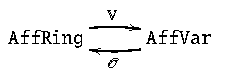
\includegraphics[width=0.48\textwidth]{figures/Fig_101_PDF188_Book176.pdf}
  \caption{仿射环与仿射簇之间的反等价（原书 p.176）}
  \label{fig:affring-affvar-antiequivalence}
\end{figure}

\subsection{模作为层}\label{subsec:modules-as-sheaves}
设 $R$ 是仿射环，$g\in R$。态射 $\iota\colon R\to R[g^{-1}]$ 诱导映射 $V(\iota)\colon V(R[g^{-1}])\to V(R)$。该映射是一个嵌入，其像为
\[
  U_g=\{\rho\in V(R)\mid \rho(g)\ne0\}.
\]
这类子集称为仿射开集\index{fangshekaiji@仿射开集|hyperpage}，它们生成 $X=V(R)$ 上的一种拓扑，称为 Zariski 拓扑\index{zariskituopu@Zariski 拓扑|hyperpage}。注意，两个仿射开集的交仍是仿射开集，且 $U_g\cap U_h=U_{gh}$；但仿射开集的并却未必是仿射的。

\begin{definition}{开集范畴}{open-category}
范畴 $\mathrm{Open}(X)$ 的对象是 $X$ 的所有 Zariski 开集\index{zariskikaiji@Zariski 开集|hyperpage}，态射是包含映射。仿射开集组成的全子范畴记为 $\mathrm{AffOpen}(X)$。
\end{definition}

\begin{note}\label{note:zariski-topology}
\textbf{注 7.6.} $V(R)$ 作为 $\mathbb C^n$ 子集所继承的通常拓扑，比 Zariski 拓扑精细得多。一般而言，Zariski 拓扑不是 Hausdorff 的。事实上，若 $R$ 没有零因子，则每个非空 Zariski 开集都是稠密的。
\end{note}

设 $M$ 是一个 $R$-模，$\rho\colon R\to\mathbb C$ 是 $X=V(R)$ 中一点，则张量积
\[
  M_\rho:=M\otimes_\rho\mathbb C
  =\frac{M\otimes\mathbb C}{(mr\otimes1-m\otimes\rho(r)\mid r\in R)}
\]
是一个 $\mathbb C$-向量空间。让 $\rho$ 变化，便得到一个定义在 $X$ 上的“向量丛\index{xiangliangcong@向量丛|hyperpage}”；不过，与向量丛不同，$M_\rho$ 的维数可能随 $\rho\in X$ 改变。

$M$ 中的每个元素 $m$ 都给出向量 $m\otimes1\in M_\rho$，因而可视为这个“丛”的一个截面。把它限制到仿射开集 $U_g\subset X$ 上时，$M\otimes_RR[g^{-1}]$ 中的元素可解释为局部截面，因为
\[
  m\otimes g^{-1}(\rho)=m\otimes\rho(g)^{-1}\in M_\rho.
\]
若两个仿射开集包含关系为 $U_g\subset U_h$，则 $R[h^{-1}]\subset R[g^{-1}]$，并有一个反向的限制映射
\[
  M(U_h)\longrightarrow M(U_g),\qquad
  M\otimes_RR[h^{-1}]\longrightarrow M\otimes_RR[g^{-1}].
\]
因此，$M$ 给出一个反变函子 $\mathrm{AffOpen}(X)\to\mathrm{Vect}_{\mathbb C}$（也可以取值于 $\mathrm{Mod}_R$）。回忆例\ref{ex:geometric-modules}：从 $\mathrm{Open}(X)$ 出发的反变函子称为预层\index{ceng@层|hyperpage}。若要把 $M$ 扩展为定义在整个 $\mathrm{Open}(X)$ 上的函子，就需要确定非仿射开集上的取值。其思路是把截面粘合起来。

具体地，设 $\mathcal S\colon\mathrm{Open}(X)\to\mathrm{Vect}_{\mathbb C}$ 是一个预层，令 $U=\bigcup_{i\in I}U_i$ 是开覆盖，并记 $U_{ij}=U_i\cap U_j$。由这些数据可构造两个映射
\[
  \mathcal S(U)\xrightarrow{\iota}\prod_i\mathcal S(U_i)
  \xrightarrow{\delta}\prod_{i<j}\mathcal S(U_{ij}),
\]
其中
\[
  \iota(x)=\bigl(\mathcal S(U_i\hookrightarrow U)(x)\bigr)_{i\in I},
\]
而
\[
  \delta((x_i)_{i\in I})_{ij}
  =\mathcal S(U_{ij}\hookrightarrow U_i)(x_i)
   -\mathcal S(U_{ij}\hookrightarrow U_j)(x_j).
\]
第二个映射检验局部截面 $(x_i)_{i\in I}$ 是否在交叠处彼此相容。若这些 $x_i$ 都来自 $U$ 上的一个截面，当然相容，故 $\delta\iota=0$。但可能存在属于 $\ker\delta$ 却不属于 $\operatorname{im}\iota$ 的元素；这说明 $\mathcal S(U)$ 中缺少某些截面。

\begin{definition}{层}{sheaf}
若对每个开覆盖 $U=\bigcup_{i\in I}U_i$，都有 $\ker\delta=\operatorname{im}\iota$，则称预层 $\mathcal S\colon\mathrm{Open}(X)\to\mathrm{Vect}_{\mathbb C}$ 为一个层。
\end{definition}

\begin{lemma}{模预层的层化}{module-presheaf-sheaf}
函子 $M\colon\mathrm{AffOpen}(X)\to\mathrm{Vect}_{\mathbb C}$ 可以扩展为层 $M\colon\mathrm{Open}(X)\to\mathrm{Vect}_{\mathbb C}$。
\end{lemma}
\begin{proof}[证明思路]
对任意开集 $U$，取所有包含于 $U$ 的仿射开集作为覆盖，并定义 $M(U)$ 为相应映射 $\delta$ 的核。
\end{proof}

\begin{example}[仿射平面上的非仿射开集]
考察仿射平面 $\mathbb A^2=V(R)$，其中 $R=\mathbb C[X,Y]$。开集
\[
  U=U_X\cup U_Y=\mathbb A^2\setminus\{(0,0)\}
\]
不是仿射开集。取 $M=R$，则 $M(U)$ 中的局部截面对应于一对函数
\[
  (f(X,Y),g(X,Y))\in M(U_X)\times M(U_Y)
  =R[X^{-1}]\times R[Y^{-1}],
\]
它们在 $M(U_{XY})=R[X^{-1},Y^{-1}]$ 中相等。这意味着 $f$ 不含 $X$ 的负次幂，$g$ 不含 $Y$ 的负次幂；因而二者都属于 $R$。所以 $M(U)\cong R$。
\end{example}

\begin{definition}{拟相干层与相干层}{quasicoherent-coherent-sheaf}
若层 $M\colon\mathrm{Open}(X)\to\mathrm{Vect}_{\mathbb C}$ 来自某个 $R$-模 $M$，则称其为拟相干层\index{xiangganceng@相干层|hyperpage}\index{nixiangganceng@拟相干层|hyperpage}；若 $M$ 有限生成，则称其为相干层。
\end{definition}

\begin{example}[点上的点层]
设一维模 $M=\mathbb C$ 上的 $R$-作用由表示 $\sigma\colon R\to\mathbb C$ 给出。向量空间 $M_\rho$ 在 $\rho=\sigma$ 时为一维，在其他情形下为零维。同样，$M$ 在 $U_g$ 上的截面空间，当且仅当 $\sigma\in U_g$ 时为一维，否则为零维。对非仿射开集也如此。这个相干层 $M$ 称为支撑在 $\sigma$ 上的点层。
\end{example}

\begin{example}[秩一自由层]
若 $M=R$，那么对 $V(R)$ 中每个点 $\rho$，向量空间 $M_\rho$ 都是一维；而 $U_g$ 上的截面空间为 $\mathcal O(U_g)=R[g^{-1}]$。相干层 $M$ 称为秩一自由层\index{zhiyiziyouceng@秩一自由层|hyperpage}，它表示 $V(R)$ 上的平凡秩一向量丛。
\end{example}

\begin{definition}{结构层}{structure-sheaf}
秩一自由层还可以看作一个环层\index{huanceng@环层|hyperpage}，因为每个 $\mathcal O(U)$ 都有环结构。把它称为 $X$ 的结构层\index{jiegouceng@结构层|hyperpage}，记作 $\mathcal O_X$。若 $M$ 是任意 $R$-模，则层 $M$ 是一个 $\mathcal O_X$-模层\index{oxmoceng@O\_X-模层|hyperpage}：对每个开集 $U$，$M(U)$ 都是 $\mathcal O_X(U)$-模。
\end{definition}

\subsection{粘合簇}\label{subsec:gluing-varieties}
正如可以把 $\mathbb R^n$ 的不同开片粘合成流形，我们也可以尝试把不同仿射簇粘合成更大的簇。先取一个空间 $X=U_1\cup\cdots\cup U_r$，使每个 $U_i$ 都是仿射簇，其坐标环为 $R_i=\mathcal O(U_i)$，并且任意交集 $U_{ij}=U_i\cap U_j$ 都是 $U_i$ 与 $U_j$ 中的仿射开集。交集的坐标环
\[
  R_{ij}:=\mathcal O(U_{ij})
\]
可写成 $R_i[g_{ij}^{-1}]$ 与 $R_j[g_{ji}^{-1}]$，其中 $g_{ij}\in R_i$、$g_{ji}\in R_j$ 是某些函数。于是得到限制态射
\[
  R_i\longrightarrow R_i[g_{ij}^{-1}]
  =R_{ij}=R_j[g_{ji}^{-1}]\longleftarrow R_j.
\]

固定这些数据之后，对高阶交集 $U_{i_1\cdots i_k}$ 也可定义坐标环
\[
  R_{i_1\cdots i_k}
  =R_{i_1}[g_{i_1i_2}^{-1},\ldots,g_{i_1i_k}^{-1}],
\]
并对所有包含关系 $U_{j_1\cdots j_\ell}\subset U_{i_1\cdots i_k}$ 定义限制态射
\[
  R_{i_1\cdots i_k}\longrightarrow R_{j_1\cdots j_\ell}.
\]

所有 $U_i$ 中的仿射开集生成 $X$ 上的 Zariski 拓扑；同样可以定义范畴 $\mathrm{Open}(X)$。空间 $X$ 带有一个自然的环层 $\mathcal O_X$，称为结构层，并满足
\[
  \mathcal O_X(U_{i_1\cdots i_k})=R_{i_1\cdots i_k}.
\]
每个开集 $U_i$ 都有一个全忠实嵌入 $\iota_i\colon\mathrm{Open}(U_i)\hookrightarrow\mathrm{Open}(X)$，而 $\mathcal O_X\circ\iota_i$ 就是 $U_i$ 上的结构层 $\mathcal O_{U_i}$。

\begin{definition}{带仿射覆盖的簇}{variety-affine-cover}\index{daifangshefugaidecu@带仿射覆盖的簇|hyperpage}
二元组 $(X,\mathcal O_X)$ 称为一个簇，其仿射覆盖为 $\mathcal U=\{U_1,\ldots,U_r\}$。\footnote{与流形的情形类似，为使一切良好，还需要对覆盖施加一些额外条件（例如分离性），这里不再讨论。}
\end{definition}

\begin{example}[射影空间]
射影空间 $\mathbb P^n$ 由 $\mathbb C^{n+1}$ 的所有一维子空间组成。我们用 $(x_0:\cdots:x_n)\in\mathbb P^n$ 表示子空间 $\mathbb C(x_0,\ldots,x_n)\subset\mathbb C^{n+1}$。它可由 $n+1$ 个开集覆盖：
\[
  U_i=\{(x_0:\cdots:x_n)\mid x_i\ne0\}
  =\left\{\left(\frac{x_0}{x_i}:\cdots:1:\cdots:\frac{x_n}{x_i}\right)\right\}
  \cong\mathbb C^n.
\]
坐标环 $\mathcal O(U_i)$ 可识别为多项式环 $\mathbb C[\xi_{ki}\mid k\ne i]$，其中 $\xi_{ki}$ 表示有理函数 $X_k/X_i$。在交叠处有嵌入
\[
  \mathbb C[\xi_{ki}\mid k\ne i]
  \longrightarrow \mathbb C[\xi_{ki}\mid k\ne i][\xi_{ji}^{-1}]
  =\mathbb C[\xi_{k\ell}\mid \ell=i,j]
  =\mathbb C[\xi_{kj}\mid k\ne j][\xi_{ij}^{-1}]
  \longleftarrow\mathbb C[\xi_{kj}\mid k\ne j].
\]
这足以计算 $\mathbb P^n$ 上的结构层：一般地，对 $\mathrm{Open}(\mathbb P^n)$ 中任意开集 $U$，有
\[
  \mathcal O(U)=\left\{\frac fg\in\mathbb C(X_0,\ldots,X_n)
  \ \middle|\ \deg f=\deg g,\ g(x)\ne0\text{ 对每个 }x\in U\right\}.
\]
第一个条件保证 $f/g$ 的值不依赖于代表元 $(x_0:\cdots:x_n)$；第二个条件保证 $f/g$ 在 $U$ 上有定义。
\end{example}

\begin{example}[射影簇与拟射影簇]
更一般地，设
\[
  R=\mathbb C[X_0,\ldots,X_n]/(f_1,\ldots,f_k)
\]
是正分次仿射整环（即 $\deg X_i\ge0$，且 $f_i$ 都是齐次元）。定义
\[
  U_i=V\bigl((R[X_i^{-1}])_0\bigr),
\]
并用包含关系
\[
  (R[X_i^{-1}])_0\longrightarrow
  (R[X_i^{-1},X_j^{-1}])_0\longleftarrow(R[X_j^{-1}])_0
\]
把这些开集粘合。由此得到的空间记作 $\mathbb P(R)$。
\end{example}

若 $R=\mathbb C[X_0,\ldots,X_n]$ 且所有 $X_i$ 的次数都是 $1$，则 $\mathbb P(R)=\mathbb P^n$。对次数均为 $1$ 的更一般的环 $R=\mathbb C[X_0,\ldots,X_n]/(f_1,\ldots,f_k)$，可将 $\mathbb P(R)$ 识别为
\[
  X=\{(x_0:\cdots:x_n)\in\mathbb P^n\mid f_i(x_0,\ldots,x_n)=0\}.
\]
这类簇称为射影簇\index{sheyingcu@射影簇|hyperpage}。若 $R$ 是多项式环，其中 $X_0,\ldots,X_k$ 的次数为 $1$，其余变量的次数为 $0$，则 $\mathbb P(R)=\mathbb P^k\times\mathbb A^{n-k}$。加入关系会截出子簇，称为拟射影簇\index{nisheyingcu@拟射影簇|hyperpage}。注意，并非所有簇都属于这一类。

直观地说，$(X,\mathcal O_X)$ 上的拟相干层应当是这样一种层：在局部看起来像仿射开集上的拟相干层。

\begin{definition}{簇上的（拟）相干层}{coherent-sheaf-on-variety}
若 $\mathcal O_X$-模层 $M$ 满足：对每个仿射开集 $U\subset X$，限制 $M|_{\mathrm{Open}(U)}$ 都是 $\mathcal O_U$ 上的拟相干层，则称 $M$ 为（拟）相干层。
\end{definition}

只需在一个仿射覆盖上检验上述条件。因此，要在 $X=\bigcup_iU_i$ 上构造拟相干层，需要给出以下数据：
\begin{itemize}
  \item 对每个 $U_i$，给出一个 $R_i$-模 $M_i$；
  \item 对每个 $U_{ij}$，给出一个 $R_{ij}$-模 $M_{ij}$ 和 $R_{ij}$-模同构
  \[
    M_i\otimes_{R_i}R_{ij}\xrightarrow{\pi_{ij}}M_{ij}
    \xleftarrow{\pi_{ji}}M_j\otimes_{R_j}R_{ij}.
  \]
\end{itemize}
这些数据给出 $U_i$ 上的拟相干层 $M_i$、$U_{ij}$ 上的拟相干层 $M_{ij}$ 和自然变换 $\pi_{ij}\colon M_i|_{\mathrm{Open}(U_{ij})}\to M_{ij}$。这些变换必须满足相容关系，才能在更高阶交集上作良好定义。\footnote{把这个相容条件明确写出来，是一道很好的练习。}固定所有这些数据后，对 $X$ 上的层 $M$ 定义
\[
  M(V)=\ker\delta,
\]
其中对每个开集 $V\subset X$，有映射
\[
  \begin{aligned}
  \delta\colon\prod_iM_i(V_i)&\longrightarrow\prod_{i<j}M_{ij}(V_{ij}),\\
  (x_i)_i&\longmapsto
  \bigl(\pi_{ij}M_i(V_{ij}\hookrightarrow V_i)(x_i)
       -\pi_{ji}M_j(V_{ij}\hookrightarrow V_j)(x_j)\bigr)_{ij},
  \end{aligned}
\]
这里 $V_i=V\cap U_i$，$V_{ij}=V\cap U_i\cap U_j$。换言之，$V$ 上的截面是各个 $V_i$ 上截面的粘合。由于 $\mathcal O_X(V)$ 的截面也以类似方式构造，可以证明 $M(V)$ 是 $\mathcal O_X(V)$-模，故 $M$ 是 $X$ 上的拟相干层。

\begin{example}[射影簇上的层与分次模]
设
\[
  R=\mathbb C[X_0,\ldots,X_n]/(f_1,\ldots,f_k)
\]
是正分次整环，$M$ 是一个 $\mathbb Z$-分次 $R$-模。在 $X=\mathbb P(R)$ 上定义层
\[
  M(U_{X_i})=(M\otimes_RR[X_i^{-1}])_0,
\]
并使用标准映射
\[
  (M\otimes_RR[X_i^{-1}])_0\longrightarrow
  (M\otimes_RR[X_i^{-1},X_j^{-1}])_0
  \longleftarrow(M\otimes_RR[X_j^{-1}])_0
\]
来粘合。取 $M=R$ 时得到 $\mathbb P(R)$ 上的结构层。若取 $M=R(k)$，其中 $R(k)_i=R_{i+k}$，则当 $k\ne0$ 时，新层 $\mathcal O(k)$ 不等于结构层 $\mathcal O$，因为它们的截面不同：
\[
  \mathcal O(k)(U_i)=R[X_i^{-1}]_k,
  \qquad \mathcal O(k)(\mathbb P^n)=R_k.
\]

不同的分次模可能给出相同的层。若 $M$ 是有限维 $R$-模，则当 $n$ 充分大时 $X_i^nM=0$，从而 $M\otimes_RR[X_i^{-1}]=0$。因此每个 $M(U_i)$ 都为零，故 $M$ 给出零层。类似地，若 $M$ 含有有限维分次子模 $N$，那么 $M$ 与 $M/N$ 所给出的层相同。

反过来，若 $M$ 是 $\mathbb P(R)$ 上的层，可以构造一个相应的分次模。先定义层 $M(k)$，使得对每个仿射开集 $U_i$，
\[
  M(k)(U_i)=M(U_i)\otimes_{\mathcal O(U_i)}\mathcal O(k)(U_i),
\]
再令
\[
  \widetilde M=\bigoplus_{k\ge0}M(k)(X).
\]
可以验证，$\widetilde M$ 所对应的层同构于原来的 $M$，因为它们在每个 $U_i$ 及其交集上都相同。
\end{example}

\subsection{层上同调}\label{subsec:sheaf-cohomology}
设簇 $(X,\mathcal O_X)$ 上有拟相干层 $M$，并取仿射覆盖 $\mathcal U=\{U_1,\ldots,U_r\}$。记
\[
  M_{i_1\cdots i_k}:=M(U_{i_1}\cap\cdots\cap U_{i_k}).
\]
前面已经看到，为构造整体截面，需要取一个衡量各个交叠上差异的映射 $\delta$ 的核。这个映射实际上是一个复形的首个微分。

\begin{definition}{Čech 复形}{cech-complex}
层 $M$ 关于覆盖 $\mathcal U$ 的 Čech 复形为
\[
  C^k_{\check C}(M,\mathcal U)
  =\bigoplus_{i_1<\cdots<i_k}M_{i_1\cdots i_k},
\]
其微分为
\[
  d^k=\sum_{i_1<\cdots<i_{k+1}}\sum_{j=1}^{k+1}
  (-1)^j\,[M_{i_1\cdots\widehat{i_j}\cdots i_{k+1}}
  \longrightarrow M_{i_1\cdots i_{k+1}}],
\]
其中求和遍历所有限制映射。
\end{definition}

该复形的零次上同调由所有整体截面组成：
\[
  H^0_{\check C}(M,\mathcal U)=M(X).
\]
这个空间不依赖于具体选取的覆盖，而只取决于层本身；更高阶上同调群也具有这一性质。

\begin{lemma}{Čech 上同调与仿射覆盖无关}{cech-cover-independence}
Čech 复形的上同调与仿射覆盖的选取无关。
\end{lemma}
\begin{proof}[证明思路]
由 Serre 定理，若仿射覆盖 $\mathcal U'$ 是覆盖 $\mathcal U$ 的细化，则 $C^\bullet_{\check C}(M,\mathcal U')$ 与 $C^\bullet_{\check C}(M,\mathcal U)$ 拟同构。此外，任意两个仿射覆盖都有一个共同细化。
\end{proof}

\begin{example}[射影空间上的线丛上同调]\label{ex:projective-space-cohomology}
令 $X=\mathbb P^n=\mathbb P(R)$，其中 $R=\mathbb C[X_0,\ldots,X_n]$，并取 $M=\mathcal O(k)$。此时 $M_{i_1\cdots i_\ell}$ 是 $R[X_{i_1}^{-1},\ldots,X_{i_\ell}^{-1}]$ 中所有 $k$ 次齐次函数组成的空间，限制映射是标准嵌入。复形 $C^\bullet_{\check C}(M,\mathcal U)$ 按单项式 $m=X_0^{s_0}\cdots X_n^{s_n}$ 分解。对每个单项式，在 $M_{i_1\cdots i_\ell}$ 中，当且仅当所有负幂变量 $X_j$ 的下标都属于 $\{i_1,\ldots,i_\ell\}$ 时，对应部分才是一维向量空间。

以 $\mathbb P^2$ 为例，一般的复形如下图所示：
\begin{figure}[H]\centering
  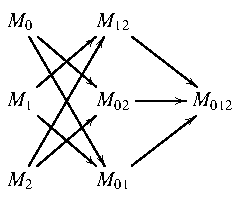
\includegraphics[width=0.54\textwidth]{figures/Fig_102_PDF194_Book182.pdf}
  \caption{三开覆盖的 Čech 复形（原书 p.182）}
  \label{fig:cech-complex-p2}
\end{figure}

根据单项式中负次幂变量的个数，共有四种情形。每出现一个负幂变量 $X_i$，就要删去所有下标中不含 $i$ 的 $M$ 项。各情形所得子复形及其上同调如下图所示：
\begin{figure}[H]\centering
  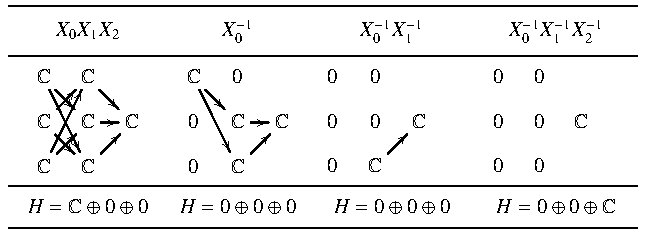
\includegraphics[width=0.96\textwidth]{figures/Fig_103_PDF194_Book182.pdf}
  \caption{按负次幂单项式分解 Čech 复形（原书 p.182）}
  \label{fig:cech-monomial-summands}
\end{figure}
由此可得
\[
  H^i_{\check C}(\mathcal O(k),\mathcal U)=
  \begin{cases}
    R_k, & i=0,\\
    0, & i=1,\\
    \left\langle X_0^{-r}X_1^{-s}X_2^{-t}\ \middle|\ 
    r,s,t\ge1,\ k=-r-s-t\right\rangle, & i=2.
  \end{cases}
\]
\end{example}

\begin{note}\label{note:projective-space-cohomology-range}
\textbf{注 7.21.} 只有 $k\ge0$ 时 $H^0$ 才可能非零，只有 $k\le-3$ 时 $H^2$ 才可能非零。对 $i\ne0,2$，上同调均为零。
\end{note}

\begin{definition}{局部自由层}{locally-free-sheaf}
$X$ 上的局部自由层\index{jubuziyouceng@局部自由层|hyperpage}是一个拟相干层 $\mathcal F$，并且存在一个仿射覆盖 $\mathcal U=\{U_i\mid i\in I\}$，使每个 $\mathcal F(U_i)$ 都是 $\mathcal O(U_i)$-自由模。
\end{definition}

簇上的局部自由相干层是向量丛的代数对应物。事实上，若对某个仿射开集 $U$，$\mathcal F(U)$ 是有限生成自由模，则
\[
  \mathcal F(U)\cong\mathcal O(U)^r,
\]
而对 $U$ 上每个点 $\rho$，纤维为
\[
  \mathcal F(U)_\rho=\mathcal O(U)^r_\rho=\mathbb C^r.
\]
整数 $r$ 称为秩；秩为 $1$ 时，$\mathcal F$ 称为可逆层\index{keniceng@可逆层|hyperpage}。之所以这样命名，是因为可以定义层的张量积，并在仿射开集上令
\[
  (\mathcal M\otimes\mathcal N)(U)
  :=\mathcal M(U)\otimes_{\mathcal O(U)}\mathcal N(U).
\]
在这个运算下，结构层 $\mathcal O$ 是单位元，而可逆层是具有逆元的层；其逆层由
\[
  \mathcal M^{-1}(U):=\operatorname{Hom}_{\mathcal O(U)}(\mathcal M(U),\mathcal O(U))
\]
给出。

\begin{example}[射影空间上的可逆层]
$X=\mathbb P^n$ 上的层 $\mathcal O(k)$ 都是局部自由层。令 $R=\mathbb C[X_0,\ldots,X_n]$，则
\[
  \mathcal O(U_i)=\mathbb C\left[\frac{X_0}{X_i},\ldots,\frac{X_n}{X_i}\right],
\]
并且
\[
  \mathcal O(k)(U_i)=R[X_i^{-1}]_k
  =X_i^k\mathbb C\left[\frac{X_0}{X_i},\ldots,\frac{X_n}{X_i}\right].
\]
因此，$\mathcal O(k)(U_i)$ 是秩为 $1$ 的自由 $\mathcal O(U_i)$-模。
\end{example}

\begin{example}[局部自由但非自由的模]
若 $X=V(R)$ 是仿射簇，则相干层局部自由，当且仅当它对应于一个投射模。这是 Serre--Swan 定理的代数几何版本\bookcite{222}；证明见\bookcite[Tag 00NV]{230}。下面用一个局部自由但非自由的模说明这一点。

取
\[
  R=\mathbb C[X,Y]/(Y^2-X^3+X),
\]
它给出嵌入于 $\mathbb A^2$ 的一条仿射椭圆曲线。模 $\mathcal F=RX+RY$ 不是自由模；但是对开覆盖 $X=U_X\cup U_{X^2-1}$，有
\[
\begin{aligned}
  \mathcal F(U_X)
    &=R[X^{-1}]X+R[X^{-1}]Y=R[X^{-1}],\\
  \mathcal F(U_{X^2-1})
    &=R[(X^2-1)^{-1}]X+R[(X^2-1)^{-1}]Y\\
    &=R[(X^2-1)^{-1}]Y\cong R[(X^2-1)^{-1}].
\end{aligned}
\]
故 $\mathcal F$ 是秩为 $1$ 的局部自由层。更一般地，这条曲线上任意一点所对应的极大理想 $\mathfrak p\subset R$ 都给出秩为 $1$ 的局部自由层，因为总能找到一个开覆盖，使 $\mathfrak p$ 在每个开片上成为主理想。下一节将进一步讨论这一点。
\end{example}

\begin{example}[除子所确定的层]\label{ex:divisor-sheaf}
设 $h(X,Y,Z)$ 是齐次多项式，且 $R=\mathbb C[X,Y,Z]/(h)$ 定义射影平面 $\mathbb P^2$ 中的一条光滑曲线 $X=\mathbb P(R)$。除子是 $X$ 中点的一个整系数组合：
\[
  D=a_1P_1+\cdots+a_kP_k.
\]
每个除子都定义一个层 $\mathcal O(D)$。它在仿射开集 $U$ 上的局部截面，是在每个 $P_i\in U$ 处阶数至少为 $-a_i$ 的有理函数：
\[
  \mathcal O(D)(U)=\left\{\frac fg\ \middle|\ f,g\in\mathcal O(U),\quad
  \operatorname{ord}_{P_i}(f)-\operatorname{ord}_{P_i}(g)\ge -a_i\text{ 对所有 }P_i\in U\right\}.
\]
（回忆：若 $\mathfrak p\subset\mathcal O(U)$ 是对应于点 $P$ 的极大理想，则 $\operatorname{ord}_{P}(f)$ 是满足 $f\in\mathfrak p^n$ 的最大指数 $n$。）与上一个例子类似，这些层都是秩为 $1$ 的局部自由层，也称线丛。线丛 $\mathcal O(D)$ 的次数定义为 $\sum_i a_i$。
\end{example}

给定簇 $(X,\mathcal O)$ 上的两个拟相干层 $\mathcal M,\mathcal N$，定义 Hom 层
\[
  \operatorname{Hom}(\mathcal M,\mathcal N)(U_i)
  :=\operatorname{Hom}_{\mathcal O(U_i)}(\mathcal M(U_i),\mathcal N(U_i)).
\]
这些 Hom 层可用来定义一个以层为态射对象的富集范畴\index{cengzhifanchou@层值范畴|hyperpage} $\mathrm{QCoh}\,X$，其对象是所有相干层，态射空间为相应的 Hom 层。该范畴有全子范畴 $\mathrm{Coh}\,X$ 和 $\mathrm{Vect}\,X$，分别由所有相干层与所有局部自由相干层组成。
% [Tutor Note: 原文称 $\mathrm{QCoh}\,X$ 的对象是“所有相干层”，但按记号 $\mathrm{QCoh}$ 取的应是所有拟相干层，相干层只构成其全子范畴 $\mathrm{Coh}\,X$（这正是下一句所说的全子范畴）；原书此处为笔误，勿据此记忆。]

若取一个开覆盖 $\mathcal U$，则可通过 Čech 复形构造一个 dg-范畴 $\mathrm{Vect}^{\bullet}(X;\mathcal U)$。它与 $\mathrm{Vect}\,X$ 有相同对象，而 Hom 空间为
\[
  \mathrm{Vect}^{\bullet}(X;\mathcal U)(\mathcal M,\mathcal N)
  :=C^\bullet_{\check C}\bigl(\operatorname{Hom}(\mathcal M,\mathcal N);\mathcal U\bigr).
\]
乘积使用杯积。若
\[
  f\in C^k_{\check C}(\operatorname{Hom}(\mathcal N,\mathcal P);\mathcal U),\qquad
  g\in C^\ell_{\check C}(\operatorname{Hom}(\mathcal M,\mathcal N);\mathcal U),
\]
则令
\[
  (f\smile g)_{i_0\cdots i_{k+\ell}}
  =f_{i_0\cdots i_k}|_{U_{i_0\cdots i_{k+\ell}}}
   \circ g_{i_k\cdots i_{k+\ell}}|_{U_{i_0\cdots i_{k+\ell}}}.
\]

\begin{lemma}{仿射覆盖改变下的拟等价}{vector-sheaf-cover-independence}
不同仿射覆盖给出拟等价的 $A_\infty$ 范畴 $\mathrm{Vect}^{\bullet}(X;\mathcal U)$ 与 $\mathrm{Vect}^{\bullet}(X;\mathcal U')$：
\[
  \mathrm{Vect}^{\bullet}(X;\mathcal U)\cong_\infty
  \mathrm{Vect}^{\bullet}(X;\mathcal U').
\]
\end{lemma}
\begin{proof}[证明思路]
证明与 Čech 上同调不依赖仿射覆盖的论证类似：由覆盖细化得到的拟同构与杯积相容。
\end{proof}

\begin{definition}{完美复形范畴}{perfect-complexes-variety}
$X$ 上向量丛完美复形\index{xiangliangcongwanmeifuxingfanchou@向量丛完美复形范畴|hyperpage}的范畴，定义为局部自由层 dg-范畴的导出范畴：
\[
  \mathrm{Perf}^{\bullet}X:=D\mathrm{Vect}^{\bullet}(X;\mathcal U).
\]
\end{definition}

\begin{example}[仿射簇上的完美复形]
若 $X=V(R)$ 是仿射簇，则局部自由层对应于 $R$ 的有限生成投射模。此外，可以取 $\mathcal U=\{V(R)\}$ 作为 $X$ 自身的仿射覆盖，此时 Čech 复形集中在次数 $0$。若投射 $R$-模 $P,Q$ 对应于层 $\mathcal P,\mathcal Q$，则
\[
  \mathrm{Vect}^{\bullet}(X;\mathcal U)(\mathcal P,\mathcal Q)
  =\operatorname{Hom}_R(P,Q).
\]
由此得到 $A_\infty$ 范畴等价
\[
  \mathrm{Vect}^{\bullet}(X;\mathcal U)\cong_\infty
  \mathrm{Proj}^{\bullet}R=\mathrm{SplitAdd}\,R,
\]
其中右侧视为集中在次数 $0$ 的 $A_\infty$ 范畴。取导出范畴后可得
\[
  \mathrm{Perf}^{\bullet}X\cong_\infty D\mathrm{Proj}^{\bullet}R=D^\pi R.
\]
因此 $R$ 是 $\mathrm{Perf}^{\bullet}X$ 的分裂生成元。
\end{example}

\begin{example}[射影平面上的 Beilinson 箭图]\label{ex:beilinson-quiver}
考察 $X=\mathbb P^2$，令 $R=\mathbb C[X_0,X_1,X_2]$。由于 $\mathcal O(k)$ 都是局部自由层，它们是 $\mathrm{Vect}\,X$ 中的对象，而且
\[
  \operatorname{Hom}(\mathcal O(k),\mathcal O(\ell))=\mathcal O(\ell-k).
\]
由例\ref{ex:projective-space-cohomology}中的计算可知，当 $\ell\ge k$ 时，
\[
  \mathrm{Perf}^{\bullet}X(\mathcal O(k),\mathcal O(\ell))=R_{\ell-k}
\]
集中在次数 $0$；当 $\ell-3<k<\ell$ 时，
\[
  \mathrm{Perf}^{\bullet}X(\mathcal O(k),\mathcal O(\ell))=0.
\]
取对象 $\mathcal O,\mathcal O(1),\mathcal O(2)$，可见它们之间只有次数为 $0$ 的态射，而且
\[
  \operatorname{End}_{\mathrm{Perf}^{\bullet}X}
  (\mathcal O\oplus\mathcal O(1)\oplus\mathcal O(2))
  =\begin{pmatrix}
    \mathbb C&R_1&R_2\\
    0&\mathbb C&R_1\\
    0&0&\mathbb C
  \end{pmatrix}=:B.
\]
这个代数还可以写成如下箭图及关系：
\begin{figure}[H]\centering
  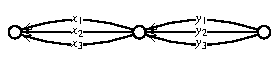
\includegraphics[width=0.52\textwidth]{figures/Fig_104_PDF197_Book185.pdf}
  \caption{Beilinson 箭图（原书 p.185）}
  \label{fig:beilinson-quiver}
\end{figure}
其中关系为 $x_i y_j=x_jy_i$。Beilinson\bookcite{26} 的著名定理说明，这三个对象生成 $\mathrm{Perf}^{\bullet}X$。因此，这个带关系的箭图称为 Beilinson 箭图\index{beilinsonjiantu@Beilinson 箭图|hyperpage}：
\[
  \mathrm{Perf}^{\bullet}X\cong_\infty
  \langle\mathcal O,\mathcal O(1),\mathcal O(2)\rangle
  \cong_\infty DB^{\bullet}.
\]
\end{example}

\subsection{光滑性}\label{subsec:smoothness}
若 $X=V(R)$ 是仿射簇，我们已经看到
\[
  \mathrm{Perf}^{\bullet}X=D\mathrm{Proj}^{\bullet}R
\]
是有界投射 $R$-模复形所成 dg-范畴 $\mathrm{TwSplitAdd}\,R$ 的极小模型。由于 $\mathrm{SplitAdd}\,R\subset\mathrm{Mod}^{\bullet}R$，有包含关系
\[
  \mathrm{Perf}^{\bullet}X\subset D\mathrm{Mod}^{\bullet}R.
\]
反过来，我们知道任意有限生成 $R$-模 $M$ 都有一个投射分解。这给出一个与 $M$ 拟同构的投射 $R$-模复形；遗憾的是，该复形未必有界，因而未必属于 $\mathrm{TwSplitAdd}\,R$。

\begin{example}[两条三次曲线]
考察两条三次曲线。
\begin{itemize}
  \item 令 $R=\mathbb C[X,Y]/(Y^2-X^3-X^2)$，并令 $S=R/(X,Y)$ 为简单模。它有如下自由分解：
  \[
  \cdots\longrightarrow R^2
  \xrightarrow{\left(\begin{smallmatrix}-X^2-X&-Y\\Y&X\end{smallmatrix}\right)}R^2
  \xrightarrow{\left(\begin{smallmatrix}-X&-Y\\Y&X^2+X\end{smallmatrix}\right)}R^2
  \xrightarrow{(Y\quad X)}R\longrightarrow S\longrightarrow0,
  \]
  且末尾这两个映射向左无限重复。由此可算得，对所有 $i>0$，$\operatorname{Ext}^i_R(S,S)=\mathbb C^2$；因此 $S$ 不可能有有界分解。
  \item 令 $R=\mathbb C[X,Y]/(Y^2-X^3+X)$，并令 $S=R/(X,Y)$ 为简单模。它有投射分解
  \[
    0\longrightarrow RX+RY\longrightarrow R\longrightarrow S\longrightarrow0.
  \]
  注意，$RX+RY$ 是投射模，但不是自由模。
\end{itemize}
从几何角度看，这两个模的区别在于：第一种情形中，$S$ 对应于 $V(R)$ 上的奇点；第二种情形中，它对应于一个光滑点。下图画出了相应的两条曲线：
\begin{figure}[H]\centering
  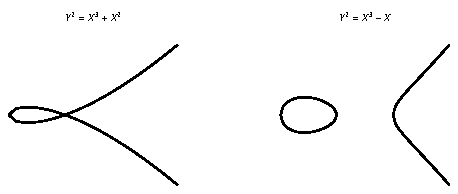
\includegraphics[width=0.66\textwidth]{figures/Fig_105_PDF198_Book186.pdf}
  \caption{奇异与光滑的三次曲线（原书 p.186）}
  \label{fig:singular-smooth-cubics}
\end{figure}
\end{example}

直观地说，光滑点 $\rho\in V(R)$ 是指它附近的空间局部看起来像仿射空间。可以通过完备化使这一说法精确化：令 $\mathfrak p=\ker\rho$，考虑
\[
  \widehat R_{\mathfrak p}=\varprojlim_i R/\mathfrak p^i.
\]
对仿射空间 $\mathbb A^n=V(\mathbb C[X_1,\ldots,X_n])$ 中的零点，有 $\mathfrak p=(X_1,\ldots,X_n)$，因此相应的完备化是形式幂级数环：
\[
  \widehat R_{\mathfrak p}\cong\mathbb C[[X_1,\ldots,X_n]].
\]
一般而言，$\widehat R_{\mathfrak p}$ 总可写成
\[
  \widehat R_{\mathfrak p}\cong\mathbb C[[X_1,\ldots,X_n]]/I,
  \qquad I\subset(X_1,\ldots,X_n)^2.
\]

\begin{definition}{光滑点}{smooth-point}
若点 $\rho\in V(R)$ 关于 $\mathfrak p=\ker\rho$ 的完备化 $\widehat R_{\mathfrak p}$ 同构于形式幂级数环 $\mathbb C[[X_1,\ldots,X_n]]$，则称 $\rho$ 是 $n$ 维光滑点。一般簇 $(X,\mathcal O_X)$ 中的点称为光滑点，如果它在某个仿射开邻域内光滑。簇光滑，当且仅当它的所有点都光滑。
\end{definition}

\begin{note}\label{note:dimension-smooth-points}
\textbf{注 7.32.} 若 $R$ 是整环，则可以证明所有光滑点都具有相同维数；这个维数称为 $V(R)$ 的维数。一般簇称为 $n$ 维的，如果它可由 $n$ 维仿射簇覆盖。
\end{note}

\begin{example}[椭圆曲线的局部完备化]
回到前面两条椭圆曲线。
\begin{itemize}
  \item 若 $R=\mathbb C[X,Y]/(Y^2-X^3+X)$，则零点处的形式完备化为
  \[
    \widehat R_{\mathfrak p}=\mathbb C[[X,Y]]/(Y^2-X^3+X).
  \]
  在该环中，$X=X^3-Y^2$，从而
  \[
    X=X^3-Y^2=(X^3-Y^2)^3-Y^2
      =((X^3-Y^2)^3-Y^2)^3-Y^2=\cdots=f(Y).
  \]
  展开后，含有 $X$ 的项次数会越来越高；极限中得到一个形式幂级数 $X=f(Y)$，所以 $\widehat R_{\mathfrak p}=\mathbb C[[Y]]$。
  \item 若 $R=\mathbb C[X,Y]/(Y^2-X^3-X^2)$，则零点处的形式完备化为
  \[
    \widehat R_{\mathfrak p}=\mathbb C[[X,Y]]/(Y^2-X^3-X^2).
  \]
  这个环不是形式幂级数环，因为它有零因子：$Y\pm X\sqrt{1+X}$ 的形式幂级数展开给出零因子分解。
\end{itemize}
\end{example}

\begin{theorem}{局部光滑性判据}{local-smoothness-criterion}
设 $R$ 是仿射整环，$X=V(R)$，$\rho\in X$ 是对应于简单 $R$-模 $S$ 的点。下列命题等价：
\begin{enumerate}[label=(\roman*)]
  \item $\rho$ 是 $n$ 维光滑点；
  \item $\operatorname{Ext}^{\bullet}_R(S,S)\cong\bigwedge^{\bullet}\mathbb C^n$；
  \item $S$ 有长度为 $n$ 的有限生成投射分解。
\end{enumerate}
\end{theorem}
\begin{proof}[证明思路]
这些等价关系来自一个事实：Ext 群和分解可以局部计算，且
\[
  \operatorname{Ext}^{\bullet}_R(S,S)
  =\operatorname{Ext}^{\bullet}_{R_{\mathfrak p}}(S,S)
  \cong\bigwedge^{\bullet}\mathbb C^n.
\]
更多信息见\bookcite[第 19 章]{74}。
\end{proof}

命题 (iii) 可以用范畴语言改述：点光滑，当且仅当 $S$ 在 $\mathrm{Perf}^{\bullet}X\subset D\mathrm{Mod}^{\bullet}R$ 中与某个对象等价。这个局部观察有一个漂亮的整体版本。

\begin{theorem}{整体光滑性判据：仿射情形}{global-smoothness-affine}
设 $R$ 是仿射整环，$X=V(R)$。下列命题等价：
\begin{enumerate}[label=(\roman*)]
  \item 簇 $X$ 光滑；
  \item 包含 $\mathrm{Perf}^{\bullet}X\subset D\mathrm{Mod}^{\bullet}R$ 是等价；
  \item $D\mathrm{MOD}^{\bullet}R$ 中的 Hom 空间次数有界，即当 $|i|\gg0$ 时，对所有 $M,N$ 都有 $D\mathrm{MOD}^{i}R(M,N)=0$。
\end{enumerate}
\end{theorem}
\begin{proof}[证明思路]
代数几何中的标准事实是：$V(R)$ 为 $n$ 维光滑簇\index{guanghuacu@光滑簇|hyperpage}，当且仅当每个 $R$-模 $M$ 都有长度至多为 $n$ 的投射分解\bookcite[\href{https://stacks.math.columbia.edu/tag/065U}{Tag 065U}]{230}。若 $M$ 有限生成，该分解也可取为有限生成的，因而每个有限生成模都属于 $\mathrm{Perf}^{\bullet}X$。

对任意模，这意味着当 $i>n$ 或 $i<0$ 时，
\[
  \mathrm{MOD}^{i}R(M,N)=\operatorname{Ext}^{i}_R(M,N)=0.
\]
允许扭曲复形后，这些次数可以整体平移有限距离；但每个扭曲复形只有有限个直和项，所以 $\mathrm{Tw}\,\mathrm{MOD}^{\bullet}R$ 与 $D\mathrm{MOD}^{\bullet}R$ 中的 Hom 空间次数仍然有界。
\end{proof}

到目前为止，我们只考察了仿射簇。若要把上述结果推广到一般簇，就需要为 $D\mathrm{Mod}^{\bullet}R$ 和 $D\mathrm{MOD}^{\bullet}R$ 找到合适的对应物。回忆第二章：我们通过以自由分解替换每个模，构造了 $\mathrm{Mod}^{\bullet}R$ 这一 $A_\infty$ 范畴。类似地，这里应当用局部自由层的分解来替换每个相干层。

\begin{definition}{层的复形与局部自由分解}{complex-of-sheaves}
$X$ 上的层复形是一个图表
\[
  P^{\bullet}=\cdots\longrightarrow\mathcal F^{-1}
  \xrightarrow{d^{-1}}\mathcal F^0
  \xrightarrow{d^0}\mathcal F^1
  \xrightarrow{d^1}\mathcal F^2\longrightarrow\cdots,
\]
其中 $d^i\in\operatorname{Hom}(\mathcal F^i,\mathcal F^{i+1})(X)$，且对每个仿射开集 $U\subset X$，限制 $P^{\bullet}(U)$ 都是 $\mathcal O(U)$-模复形。若对每个仿射开集 $U$，$P^{\bullet}(U)$ 都是 $\mathcal M(U)$ 的投射分解，则称 $P^{\bullet}$ 是层 $\mathcal M$ 的局部自由分解。
\end{definition}

若 $P^{\bullet},Q^{\bullet}$ 分别是层 $\mathcal M,\mathcal N$ 的分解，就像前面一样，可以定义它们之间的 Hom 层 $\operatorname{Hom}(P^{\bullet},Q^{\bullet})$。对每个仿射开集 $U$，$\operatorname{Hom}(P^{\bullet},Q^{\bullet})(U)$ 是一个复形，其微分由 $P^{\bullet}$ 和 $Q^{\bullet}$ 的微分诱导。取该 Hom 层的 Čech 复形：
\[
  C^\bullet_{\check C}(\operatorname{Hom}(P^{\bullet},Q^{\bullet});\mathcal U)
  :=\bigoplus_{k,\ell}\bigoplus_{i_1,\ldots,i_k}
  \operatorname{Hom}^{\ell}(P^{\bullet},Q^{\bullet})(U_{i_1\cdots i_k}).
\]
这个双复形带有两个微分：Čech 微分 $d_C$ 提高 $k$ 次数，Hom 微分 $d_H$ 提高 $\ell$ 次数。二者反交换，所以总微分
\[
  d_T=d_C+d_H
\]
是关于 $k+\ell$ 次数的微分，因为
\[
  d_T^2=d_C^2+d_Cd_H+d_Hd_C+d_H^2=0.
\]
不同的局部自由分解和仿射覆盖给出拟同构的复形；其零次上同调是 $\mathcal M$ 与 $\mathcal N$ 的 Hom 层的整体截面：
\[
  H^0C^\bullet_{\check C}(\operatorname{Hom}(P^{\bullet},Q^{\bullet});\mathcal U)
  =\operatorname{Hom}(\mathcal M,\mathcal N)(X).
\]

\begin{definition}{层的导出范畴}{derived-categories-of-sheaves}
以拟相干层的局部自由分解为对象、以上述 Čech 复形为 Hom 空间的范畴，在总微分下构成一个 dg-范畴。记其极小模型为 $\mathrm{Coh}^{\bullet}X$（$\mathrm{QCoh}^{\bullet}X$），并记其导出版本为 $D\mathrm{Coh}^{\bullet}X$（$D\mathrm{QCoh}^{\bullet}X$）。后者称为（拟）相干层的有界导出范畴\index{xianggancengdeyoujiedaochufanchou@相干层的有界导出范畴|hyperpage}。
\end{definition}

由于 $\mathrm{Vect}^{\bullet}X$ 中每个对象都是自身的分解，存在包含
\[
  \mathrm{Vect}^{\bullet}X\subset\mathrm{Coh}^{\bullet}X
  \subset\mathrm{QCoh}^{\bullet}X.
\]
取导出范畴后得到以下两列 $A_\infty$ 范畴：
\[
\begin{array}{ll}
  \text{仿射情形:}&\mathrm{Perf}^{\bullet}X\subset D\mathrm{Mod}^{\bullet}R
    \subset D\mathrm{MOD}^{\bullet}R,\\
  \text{一般情形:}&\mathrm{Perf}^{\bullet}X\subset D\mathrm{Coh}^{\bullet}X
    \subset D\mathrm{QCoh}^{\bullet}X.
\end{array}
\]
有了这些定义，就可以把前面的定理推广到一般情形。

\begin{theorem}{整体光滑性判据：一般情形}{global-smoothness-general}
设 $X$ 是一个簇。下列命题等价：
\begin{enumerate}[label=(\roman*)]
  \item 簇 $X$ 光滑；
  \item 包含 $\mathrm{Perf}^{\bullet}X\subset D\mathrm{Coh}^{\bullet}X$ 是等价；
  \item $D\mathrm{QCoh}^{\bullet}X$ 中的 Hom 空间次数有界。
\end{enumerate}
\end{theorem}
% [Tutor Note: 光滑性判据的几何含义：$\mathrm{Perf}^{\bullet}X$ 是“由向量丛生成的有限复形”，$D\mathrm{Coh}^{\bullet}X$ 是全体有界复形；$X$ 光滑时二者相等（每个相干层都有有限局部自由分解），$X$ 有奇点时商 $D^b\mathrm{Coh}X/\mathrm{Perf}X$ 非零，它只探测奇点，这正是 §7.2.5 的奇点范畴 $\operatorname{Sing}X$。]

\begin{note}\label{note:projective-derived-hom-finite}
\textbf{注 7.39.} 若进一步假设 $X$ 是射影簇，则 $D\mathrm{Coh}^{\bullet}X$ 中的 Hom 空间不仅次数有界，而且有限维。换言之，$D\mathrm{Coh}^{\bullet}X$ 是 Hom 有限的 $A_\infty$ 范畴。
\end{note}

光滑簇自然带有一组局部自由层，它们是微分几何中相应对象的代数类比。

\begin{definition}{切层、余切层与典范层}{tangent-cotangent-canonical-sheaves}
设 $(X,\mathcal O)$ 是一个簇。
\begin{itemize}
  \item 切层\index{qieceng@切层|hyperpage} $T$ 定义为 $X$ 上的导子层：
  \[
    T(U):=\operatorname{Der}(\mathcal O(U))
    =\{\delta\colon\mathcal O(U)\to\mathcal O(U)\mid
    \delta(uv)=\delta(u)v+u\delta(v)\}.
  \]
  \item 余切层\index{yuqieceng@余切层|hyperpage} $T^*$ 定义为切层的对偶：
  \[
    T^*(U):=\operatorname{Hom}_{\mathcal O(U)}(T(U),\mathcal O(U)).
  \]
  对 $f,g\in\mathcal O(U)$，表达式 $f\,dg$ 可视为 $T^*(U)$ 中的元素，具体由 $f\,dg(\delta)=f\delta(g)$ 给出。
  \item 微分 $k$-形式层 $\Omega^\bullet$ 是余切层关于结构层的外代数：
  \[
    \Omega^\bullet(U):=\bigwedge^\bullet T^*(U)
    =\frac{\displaystyle\bigoplus_{n=0}^{\infty}T^*(U)^{\otimes n}}
      {\langle u\otimes v-v\otimes u\mid u,v\in T^*(U)\rangle}.
  \]
  \item 典范层\index{dianfanceng@典范层|hyperpage}是最高次微分形式层\index{weifenxingshiceng@微分形式层|hyperpage}：
  \[
    K(U):=\Omega^n(U),\qquad n=\dim X.
  \]
\end{itemize}
\end{definition}

\begin{theorem}{光滑簇上的向量丛}{vector-sheaves-smooth}
若 $(X,\mathcal O)$ 光滑，则 $T,T^*$ 和 $\Omega^k$ 都是局部自由层，且 $K$ 是线丛。
\end{theorem}
\begin{proof}[证明思路]
参见\bookcite[\href{https://stacks.math.columbia.edu/tag/05D4}{Tag 05D4}]{230}。
\end{proof}

\begin{example}[射影空间的典范丛]
若 $X=\mathbb P^1$，则在 $U_0$ 上可用坐标 $\xi=X/Y$ 局部写出导子 $f(\xi)\,\frac d{d\xi}$。在 $U_1$ 上令 $\eta=Y/X=\xi^{-1}$，则
\[
  f(\xi)\frac d{d\xi}
  =-f(\eta^{-1})\eta^2\frac d{d\eta}.
\]
因此，当 $f$ 的次数不超过 $2$ 时，该导子可在整体上定义，故 $T(X)=\mathbb C^3$，且 $T=\mathcal O(2)$。另一方面，由 $d\xi=-\eta^{-2}d\eta$ 可知
\[
  T^*=\Omega^1=K=\mathcal O(-2).
\]
一般地，可以证明 $\mathbb P^n$ 的典范丛为 $K=\mathcal O(-n-1)$，因为
\[
  d\xi_{10}\wedge\cdots\wedge d\xi_{n0}
  =\pm\xi_{01}^{-n-1}
  d\xi_{01}\wedge\cdots\wedge d\xi_{n1}.
\]
\end{example}

\section{其他几何对象}\label{sec:other-geometrical-objects}
\takeaway{支撑层、概形、非交换簇与栈把导出范畴推广到更广的对象；Landau--Ginzburg 模型 $(X,W)$ 的矩阵分解由 $d_0d_1=d_1d_0=W$ 刻画，Knörrer 周期性、Dyckerhoff 生成定理与 Buchweitz 定理把 $\mathrm{MF}^{\pm}(R,W)$ 与 $W^{-1}(0)$ 的奇点范畴联系起来。}
本节考察代数几何中的其他一些对象。与簇类似，我们也可以构造仿射版本和非仿射版本；后者由粘合仿射片得到，但这里不详细展开。

\subsection{支撑}\label{subsec:support}
设 $X$ 是仿射簇，$I$ 是 $R=\mathcal O(X)$ 中的理想，并假设 $R/I$ 是仿射整环。则有自然嵌入
\[
  Y=V(R/I)\hookrightarrow X,
\]
其像是 $X$ 的闭子集。若 $M$ 是 $R/I$-模，也可以把它看作 $R$-模。由此得到嵌入
\[
  \mathrm{Coh}\,Y\subset\mathrm{Coh}\,X,
\]
其中右侧的子范畴由所有支撑在 $Y$ 上的 $X$-层组成。

作为普通范畴，这是一个全忠实嵌入；但加入额外的 $A_\infty$ 结构后，情形便不再如此。事实上，若 $Y=\{p\}$ 是 $X=\mathbb A^1$ 中的一个点，则简单模 $S_p$ 作为 $\mathcal O(Y)$-模的 $A_\infty$ 自同态环为
\[
  \operatorname{Ext}^{\bullet}_{\mathbb C}(S_p,S_p)=\mathbb C,
\]
而作为 $\mathcal O(X)$-模时则为
\[
  \operatorname{Ext}^{\bullet}_{\mathbb C[X]}(S_p,S_p)
  =\mathbb C\langle\xi\rangle/(\xi^2).
\]

\begin{definition}{支撑在闭子簇上的导出范畴}{derived-category-support}
$X$ 上支撑在 $Y$ 上的相干层导出范畴记为 $D\mathrm{Coh}^{\bullet}_Y(X)$；它是 $D\mathrm{Coh}^{\bullet}(X)$ 的 $A_\infty$ 子范畴，由把 $Y$ 上的层视为 $X$ 上的层后所生成。
\end{definition}

\begin{example}[光滑点的无穷小邻域]
若 $Y=\{p\}$ 是簇 $X$ 中一个 $n$ 维光滑点，则 $D\mathrm{Coh}^{\bullet}_Y(X)$ 由点层 $S_p$ 生成。这意味着 $D\mathrm{Coh}^{\bullet}_Y(X)$ 包含 $S_p$ 的自扩张；这些扩张是 $\mathrm{Coh}\,X$ 中的层，却不属于 $\mathrm{Coh}\,Y\subset\mathrm{Coh}\,X$。

由于 $S_p$ 在 $D\mathrm{Coh}^{\bullet}(X)$ 中的自同态环是外代数 $\Lambda^\bullet_n$，我们有
\[
  D\mathrm{Coh}^{\bullet}_Y(X)\cong_\infty D\Lambda^\bullet_n.
\]
这个范畴等价于 $D\mathrm{mod}\,\mathbb C[[X_1,\ldots,X_n]]$，所以它只看见 $Y$ 在 $X$ 中的无穷小邻域。
\end{example}

\begin{note}\label{note:singular-support-in-smooth-variety}
\textbf{注 7.45.} 一般而言，若 $Y$ 是奇异的而 $X$ 光滑，则 $D\mathrm{Coh}^{\bullet}_Y(X)$ 的表现会比 $D\mathrm{Coh}^{\bullet}(Y)$ 好得多。
\end{note}

\subsection{概形}\label{subsec:schemes}
概形\index{gaixing@概形|hyperpage}是簇的推广，在这种推广中，坐标环允许是任意交换环 $R$。与 $R$ 对应的空间记作 $\operatorname{Spec}(R)$，其点由 $R$ 的所有素理想组成。$\operatorname{Spec}(R)$ 中的仿射开集具有如下形式：
\[
  U_f=\{\mathfrak p\in\operatorname{Spec}(R)\mid f\notin\mathfrak p\}.
\]
与普通簇类似，可以把 $R$ 变成 $\operatorname{Spec}(R)$ 上的环层 $\mathcal O$，令
\[
  \mathcal O(U_f)=R[f^{-1}].
\]
与 $R$ 对应的概形是带环层空间 $X=(\operatorname{Spec}(R),\mathcal O)$，并且可以按通常方式定义（拟）相干层。

若 $R$ 是仿射环，则可将 $V(R)$ 嵌入 $\operatorname{Spec}(R)$：把表示 $\rho\colon R\to\mathbb C$ 映到极大理想 $\ker\rho$。虽然 $\operatorname{Spec}(R)$ 通常比 $V(R)$ 含有更多点，但这两个拓扑空间的形态十分相似。特别地，相应的开集范畴等价：
\[
  \mathrm{Open}_{V(R)}\simeq\mathrm{Open}_{\operatorname{Spec}(R)}.
\]
因此，概形版本的 $\mathrm{Coh}^{\bullet}X$、$\mathrm{QCoh}^{\bullet}X$ 与 $\mathrm{Perf}^{\bullet}X$ 和簇版本相同，并分别等价于 $\mathrm{MOD}^{\bullet}R$、$\mathrm{Mod}^{\bullet}R$ 与 $D\mathrm{Proj}^{\bullet}R$。
% [Tutor Note: 这句的对应顺序按本书记号是反的：$MOD^{\bullet}R$ 为全部（右）模、$Mod^{\bullet}R$ 为有限生成模（见第 1 章 §1.5 的约定），故与仿射簇的对应应为 Coh$\leftrightarrow$Mod、QCoh$\leftrightarrow$MOD。原书此处把两个记号对调，对照 §7.1.4 末尾的范畴塔 $\mathrm{Coh}^{\bullet}X\subset\mathrm{QCoh}^{\bullet}X$、$D\mathrm{Mod}^{\bullet}R\subset D\mathrm{MOD}^{\bullet}R$ 即可确认。]

\begin{example}[一般点]
若 $R=\mathbb C[X]$，则 $\operatorname{Spec}(R)$ 比 $V(R)$ 多一个点，它对应素理想 $(0)$。由于 $f\notin(0)$，这个点属于每个 $U_f$，因而位于任意点的闭包中。这个点称为 $\operatorname{Spec}(R)$ 的一般点。
\end{example}

\begin{example}[胖点]
若 $R=\mathbb C[X]/(X^n)$，则 $\operatorname{Spec}(R)$ 只有一个点，即素理想 $\mathfrak p=(X)$。当 $n=1$ 时，该概形就是由一个点构成的仿射簇；当 $n>1$ 时，概形仍只有一个点，但该点附近的函数环更大，是 $R$ 而非 $\mathbb C$。因此它称为胖点\index{pangdian@胖点|hyperpage}。其导出范畴为
\[
  D\mathrm{Coh}^{\bullet}X=D\mathrm{Mod}^{\bullet}\mathbb C[X]/(X^n),
\]
它不等于 $\mathrm{Perf}^{\bullet}\mathbb C[X]/(X^n)$，所以胖点是奇异概形。
\end{example}

概形的更多内容参见\bookcite{109,184,72}。

\subsection{非交换簇}\label{subsec:noncommutative-varieties}
我们还可以尝试把视角推广到非交换环。理想情况下，希望把 $\mathrm{Mod}^{\bullet}R$ 或 $\mathrm{MOD}^{\bullet}R$ 看成某个拓扑空间上的层范畴。一般而言，这很难做到，因为“点”可能有不同的合理定义，例如素理想、极大理想、简单表示或一维表示；每种定义都有各自的缺点。通常更好的做法是完全不考虑空间，只研究范畴 $\mathrm{Mod}^{\bullet}R$、$\mathrm{MOD}^{\bullet}R$ 及其导出版本 $D\mathrm{Mod}^{\bullet}R$、$D\mathrm{MOD}^{\bullet}R$。

\begin{example}[射影空间的非交换仿射模型]
在某些情形下，射影簇可以看作仿射非交换簇。由第 4.4.2 节可知
\[
  D\mathrm{Coh}^{\bullet}\mathbb P^1
  \cong_\infty D\mathrm{mod}^{\bullet}Q
  =D\mathrm{Mod}^{\bullet}Q,
\]
其中 $Q$ 是克罗内克箭图：
\begin{figure}[H]\centering
  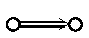
\includegraphics[width=0.30\textwidth]{figures/Fig_106_PDF204_Book192.pdf}
  \caption{克罗内克箭图（原书 p.192）}
  \label{fig:kronecker-quiver-b-side}
\end{figure}
这是因为我们找到了 $D\mathrm{Coh}^{\bullet}\mathbb P^1$ 的一个分裂生成元，其自同态环是 $Q$ 的路径代数。类似地，由例\ref{ex:beilinson-quiver}可得
\[
  D\mathrm{Coh}^{\bullet}\mathbb P^2
  \cong_\infty\mathrm{Perf}^{\bullet}\mathbb P^2
  \cong_\infty D\mathrm{Mod}^{\bullet}B,
\]
其中 $B$ 是由 Beilinson 箭图及其关系给出的路径代数。
\end{example}

若把非交换代数 $A$ 视为某个非交换簇上的函数环，把它的模视为拟相干层，就可以把几何概念转移到非交换情形。与交换簇类似，这里有三个值得关注的范畴：$D\mathrm{MOD}^{\bullet}A$ 对应 $D\mathrm{QCoh}^{\bullet}X$；有限生成模组成的 $D\mathrm{Mod}^{\bullet}A$ 对应 $D\mathrm{Coh}^{\bullet}X$；而
\[
  \mathrm{Perf}^{\bullet}A:=D\mathrm{Proj}^{\bullet}A
\]
对应 $\mathrm{Perf}^{\bullet}X$。不过，若 $A$ 不是 Noether 环，则 $D\mathrm{Mod}^{\bullet}A$ 的性质不佳，因为 $\mathrm{Mod}\,A$ 对取核不封闭。因此，下面假设 $A$ 是 Noether 环。

\begin{definition}{代数的整体维数}{global-dimension-algebra}
代数 $A$ 的（右）整体维数\index{zhengtiweishu@整体维数|hyperpage}，是使得存在 $M,N\in\mathrm{MOD}^{\bullet}A$ 满足 $\operatorname{Ext}^n_A(M,N)\ne0$ 的最大整数 $n$。若不存在这样的最大整数，则称 $A$ 的整体维数为无穷。
\end{definition}

\begin{example}[若干代数的整体维数]
列出一些重要代数的整体维数。
\begin{itemize}
  \item （斜）域的整体维数为 $0$，因为所有模都是自由模。
  \item 光滑 $n$ 维仿射簇的坐标环整体维数为 $n$。
  \item 箭图 $Q$ 的路径代数 $\mathbb C Q$ 的整体维数为 $1$，因为每个模 $M$ 都有如下分解：
  \[
    0\longrightarrow
    \bigoplus_{a\in Q_1}M_{h(a)}\otimes t(a)\mathbb C Q
    \xrightarrow{\ a\otimes t(a)-h(a)\otimes a\ }
    \bigoplus_{v\in Q_0}M_v\otimes v\mathbb C Q
    \longrightarrow M\longrightarrow0.
  \]
  \item 由 Beilinson 箭图及关系给出的路径代数，其整体维数为 $2$。
  \item 注意，整体维数不在导出等价下保持不变。下图所示的两个代数具有相同的导出范畴，但前者整体维数为 $1$，后者为 $2$：
  \begin{figure}[H]\centering
    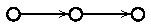
\includegraphics[width=0.33\textwidth]{figures/Fig_107_PDF205_Book193.pdf}\quad
    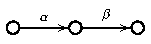
\includegraphics[width=0.37\textwidth]{figures/Fig_108_PDF205_Book193.pdf}
    \caption{导出等价但整体维数不同的代数（原书 p.193）}
    \label{fig:derived-equivalent-global-dimensions}
  \end{figure}
  \item 整体维数有限并不是一个很强的条件：每个没有有向圈的箭图所给出的带关系路径代数，都有有限整体维数。
\end{itemize}
\end{example}

\begin{theorem}{Noether 代数的光滑性判据}{smoothness-noetherian-algebra}
若 $A$ 是 Noether 环且整体维数为 $n$，则
\begin{enumerate}[label=(\roman*)]
  \item $\mathrm{Perf}^{\bullet}A\subset D\mathrm{Mod}^{\bullet}A$ 是等价；
  \item $D\mathrm{MOD}^{\bullet}A$ 中的 Hom 空间次数有界。
\end{enumerate}
\end{theorem}
\begin{proof}[证明思路]
若整体维数为 $n$，则每个模都有长度至多为 $n$ 的投射分解。由于 $A$ 是 Noether 环，这个分解可取为有限生成的，因此属于 $\mathrm{Perf}^{\bullet}A$。另一方面，我们知道模之间的 Hom 空间次数有界，所以对模的扭曲复形取 Hom 空间时，次数仍然有界。
\end{proof}

\begin{note}\label{note:noncommutative-geometry-approaches}
\textbf{注 7.52.} 把几何思想转移到非交换情形时往往不够完美，因此根据研究重点不同，存在多种非交换代数几何路径\bookcite{152,145,226}；这一领域与有限维代数表示论也有许多交叉\bookcite{97,108}。
\end{note}

\subsection{栈}\label{subsec:stacks}
设有限群 $G$ 作用在仿射簇 $X$ 上。我们希望构造一个新簇，使其点对应于 $X$ 中的轨道。为此需要找出新簇的坐标环。$G$ 在原簇上的作用诱导 $G$ 对坐标环 $R=\mathcal O(X)$ 的作用：
\[
  \forall g\in G,\ f\in R,\ x\in X,\qquad
  (g\cdot f)(x):=f(g^{-1}\cdot x).
\]
轨道集上的函数可以看成 $X$ 上在群作用下不变的函数。它们组成一个环
\[
  R^G:=\{f\in R\mid g\cdot f=f\text{ 对所有 }g\in G\},
\]
并定义商簇
\[
  X//G:=V(R^G).
\]
自然嵌入 $R^G\hookrightarrow R$ 诱导投影映射 $\pi\colon X\to X//G$；由于 $G$ 有限，$\pi$ 的纤维恰好是 $G$-轨道。

\begin{definition}{范畴商}{categorical-quotient}
簇 $X//G:=V(R^G)$ 称为范畴商\index{fanchoushang@范畴商|hyperpage}。
\end{definition}

\begin{example}[单位根作用的商]
令 $X=\mathbb A^1$，$G=\mathbb Z_n$，并令 $G$ 通过乘以 $n$ 次单位根作用。此时 $R=\mathbb C[X]$，不变函数正是关于 $X^n$ 的多项式。因此
\[
  \mathcal O(X//G)=\mathbb C[X^n],\qquad X//G\cong\mathbb A^1.
\]
\end{example}

上例表明，不变环并未完全捕捉商的几何结构：在 $X//G\cong\mathbb A^1$ 中，所有点看起来都一样，但商中有一个特殊点，即零轨道。这个轨道只含一个点，其余轨道都含 $\#G$ 个点。为解决这一问题，可以构造一个新的环。

\begin{definition}{叉积（smash product）}{smash-product}
若 $X=V(R)$ 是仿射簇，有限群 $G$ 作用在 $X$ 上，则定义叉积\index{chaji@叉积|hyperpage} $R\star G$ 为由 $R$ 与 $G$ 中元素线性组合组成的环：
\[
  R\star G:=\left\{\sum_i f_i g_i\ \middle|\ f_i\in R,\ g_i\in G\right\},
\]
其乘法满足
\[
  (f_1g_1)(f_2g_2)=\bigl(f_1(g_1\cdot f_2)\bigr)g_1g_2.
\]
\end{definition}

若 $G$ 的作用是忠实的，可以证明叉积 $R\star G$ 的中心等于不变环 $R^G$。叉积是一个非交换 $\mathbb C$-代数，因此可以将它视为一个非交换簇。

\begin{definition}{商栈}{quotient-stack}
商栈\index{shangzhan@商栈|hyperpage} $[X/G]$ 是与叉积 $R\star G$ 对应的非交换簇；按定义，
\begin{align*}
  \mathrm{Perf}^{\bullet}[X/G]&:=\mathrm{Perf}^{\bullet}(R\star G),\\
  D\mathrm{Coh}^{\bullet}[X/G]&:=D\mathrm{Mod}^{\bullet}(R\star G),\\
  D\mathrm{QCoh}^{\bullet}[X/G]&:=D\mathrm{MOD}^{\bullet}(R\star G).
\end{align*}
\end{definition}

\begin{example}[仿射直线的循环群商栈]
令 $X=\mathbb C$，$G=\mathbb Z/n\mathbb Z$，作用为乘以 $n$ 次单位根。由定理~\ref{thm:cyclic-quiver-crossed-product}，商栈对应于有 $n$ 个顶点的循环箭图路径代数：
\begin{figure}[H]\centering
  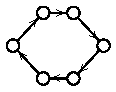
\includegraphics[width=0.28\textwidth]{figures/Fig_109_PDF206_Book194.pdf}
  \caption{循环箭图（原书 p.194）}
  \label{fig:cyclic-quiver-stack}
\end{figure}
\[
  \mathcal O(X)\star G\cong\mathbb C Q.
\]
因此
\[
  D\mathrm{Coh}^{\bullet}[X/G]\cong D\mathrm{Mod}^{\bullet}Q,
  \qquad D\mathrm{Coh}^{\bullet}(X//G)\cong D\mathrm{Mod}^{\bullet}\mathbb C[X],
\]
所以商栈确实与商簇不同。
\end{example}

从几何角度看，商栈通常比范畴商表现得更好。

\begin{example}[平面上的二阶群作用]
令 $G=\mathbb Z/2\mathbb Z\cong\{1,-1\}\cong\langle g\mid g^2=1\rangle$，并令它通过同时乘以 $-1$ 的方式对角作用在 $\mathbb A^2$ 上。$\mathbb C[X,Y]^G$ 由 $\xi=X^2$、$\eta=Y^2$、$\zeta=XY$ 生成，因此
\[
  \mathbb C[X,Y]^G\cong\mathbb C[\xi,\eta,\zeta]/(\xi\eta-\zeta^2).
\]
这表明 $X//G$ 是一个锥，并非光滑簇。另一方面，商栈 $[\mathbb A^2/G]$ 上的相干层可以看成有限生成的 $A$-模，其中
\[
  A=\mathbb C[X,Y]\star G
  =\frac{\mathbb C\langle X,Y,g\rangle}
  {(XY-YX,\ gX+Xg,\ gY+Yg,\ g^2-1)}.
\]
这个代数同构于下图所示带关系的箭图路径代数：
\begin{figure}[H]\centering
  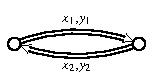
\includegraphics[width=0.43\textwidth]{figures/Fig_110_PDF207_Book195.pdf}
  \caption{商栈代数的箭图及关系（原书 p.195）}
  \label{fig:quotient-stack-quiver}
\end{figure}
其关系为
\[
  \mathcal R=\langle x_1y_2-y_1x_2,\ x_2y_1-y_2x_1\rangle.
\]
每个 $A$-模 $M$ 都有如下形式的投射分解：
\[
  0\longrightarrow M\otimes_{\mathbb CG}A
  \xrightarrow{\binom{-Y}{X}}
  (M\otimes_{\mathbb CG}A)^{\oplus2}
  \xrightarrow{(X\quad Y)}M\otimes_{\mathbb CG}A
  \longrightarrow M\longrightarrow0.
\]
\begin{figure}[H]\centering
  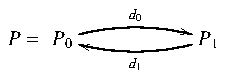
\includegraphics[width=0.62\textwidth]{figures/Fig_111_PDF207_Book195.pdf}
  \caption{叉积代数模的投射分解（原书 p.195）}
  \label{fig:quotient-stack-resolution}
\end{figure}
所以 $A$ 的整体维数为 $2$。由于 $A$ 是 Noether 环，有
\[
  D\mathrm{Coh}^{\bullet}[\mathbb A^2/G]
  \simeq\mathrm{Perf}^{\bullet}[\mathbb A^2/G].
\]
\end{example}

\begin{note}\label{note:stacks-equivariant-sheaves}
\textbf{注 7.59.} 也可以把 $[X/G]$ 上的相干层定义为 $X$ 上的 $G$-等变层。这种方法使我们能够对非仿射簇定义栈商。栈的概念甚至可以推广到不来自群作用商的情形。栈的简要介绍见\bookcite{76,196}。
\end{note}

\subsection{Landau--Ginzburg 模型}\label{subsec:landau-ginzburg-models}
矩阵分解\index{juzhenfenjie@矩阵分解|hyperpage}最初由 Eisenbud 在文献\bookcite{73}中引入，之后被物理学家用于研究某些称为 Landau--Ginzburg 模型\index{landauginzburgmoxing@Landau–Ginzburg 模型|hyperpage}的物理模型。Landau--Ginzburg 模型由一对 $(X,W)$ 组成，其中 $X$ 是一个簇，$W\colon X\to\mathbb C$ 是全纯函数。若 $X$ 是仿射簇，可以把 $W$ 看作 $\mathcal O(X)$ 中的元素；它通常称为势\index{shi@势|hyperpage}。

\begin{definition}{矩阵分解范畴}{matrix-factorization-category}
设 $(R,W)$ 是一对数据，其中 $R$ 是仿射整环，$W\in R$。
\begin{itemize}
  \item $(R,W)$ 的一个矩阵分解是一个图表
  \[
    P=P_0\underset{d_1}{\overset{d_0}{\rightleftarrows}}P_1,
    \qquad d_0d_1=W1_{P_1},\quad d_1d_0=W1_{P_0},
  \]
  其中 $P_0,P_1$ 是有限生成投射模（即 $V(R)$ 上的向量丛）。
  \item 两个矩阵分解 $P,Q$ 之间的态射空间为
  \[
    \bigoplus_{i,j\in\mathbb Z_2}\operatorname{Hom}_R(P_i,Q_j),
  \]
  微分对齐次态射 $f$ 定义为
  \[
    d\begin{pmatrix}f_{00}&f_{01}\\f_{10}&f_{11}\end{pmatrix}
    =\begin{pmatrix}0&d_1\\d_0&0\end{pmatrix}_{Q}
      \begin{pmatrix}f_{00}&f_{01}\\f_{10}&f_{11}\end{pmatrix}
      -\begin{pmatrix}f_{00}&-f_{01}\\-f_{10}&f_{11}\end{pmatrix}
       \begin{pmatrix}0&d_1\\d_0&0\end{pmatrix}_{P}.
  \]
% [Tutor Note: 微分公式右端的第二个矩阵正是 Koszul 符号：记 $\sigma=\operatorname{diag}(1,-1)$，则右端第二个矩阵等于 $\sigma f\sigma=(-1)^{|f|}f$（$f$ 为奇次时四个分量依次变号），故 $d(f)=d_Qf-(-1)^{|f|}fd_P$。漏掉这个符号 $d^2$ 一般不为零，这是矩阵分解 Hom 复形最易出错之处。]
  \item 矩阵分解范畴\index{juzhenfenjiefanchou@矩阵分解范畴|hyperpage} $\mathrm{MF}^{\pm}(R,W)$ 是以上述对象和态射为基础的 dg-范畴的极小模型。
\end{itemize}
\end{definition}

\begin{note}\label{note:matrix-factorizations-curved-algebra}
\textbf{注 7.61.} 若 $R$ 是多项式环，则 Quillen--Suslin 定理\index{quillensuslindingli@Quillen–Suslin 定理|hyperpage}\bookcite{206}说明每个投射 $R$-模都是自由模。结合例~\ref{ex:matrix-factorizations-from-potential}，可以把 $P_i$ 看成 $R^{\oplus k}$，把 $d_i$ 看成系数属于 $R$ 的矩阵。换言之，
\[
  \left(P_0\oplus P_1[1],
  \begin{pmatrix}0&d_1\\d_0&0\end{pmatrix}\right)
\]
是带曲率代数 $R_W$ 上的一个扭曲复形：
\[
  \mathrm{MF}^{\pm}(R,W)=H^0\mathrm{Tw}_{R_W}
  ={}^0\mathrm{D}R_W.
\]
\end{note}

\begin{example}[乘积势 $XY$ 的矩阵分解]
取环 $R=\mathbb C[X,Y]$ 与多项式 $W=XY$。有一个自然的矩阵分解：
\[
  S:=R\underset{Y}{\overset{X}{\rightleftarrows}}R.
\]
\begin{figure}[H]\centering
  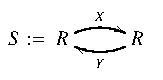
\includegraphics[width=0.23\textwidth]{figures/Fig_112_PDF208_Book196.pdf}
  \caption{$XY$ 的基本矩阵分解（原书 p.196）}
  \label{fig:xy-matrix-factorization}
\end{figure}
我们有 $\operatorname{End}_{\mathrm{MF}^{\pm}}(S,S)=\mathbb C\,1$。事实上，可以证明 $\mathrm{MF}^{\pm}(R,W)$ 由 $S$ 生成，因此它等价于 $D\mathbb C^{\pm}$，即一个点的 $\mathbb Z_2$-分次导出范畴；也就是说，它等价于矩阵分解范畴 $\mathrm{MF}^{\pm}(\mathbb C,0)$。

这并非巧合。一般而言，$\mathrm{MF}^{\pm}(R,W)$ 可用于描述零纤维
\[
  W^{-1}(0)=V(R/(W))
\]
的奇异集。对每个 $p\in W^{-1}(0)\subset\mathbb C^n$，都可以构造一个矩阵分解。设 $R=\mathbb C[X_1,\ldots,X_n]$，$p=0\in W^{-1}(0)$，并写成
\[
  W=\sum_rX_rW_r,
\]
其中 $W_r$ 是多项式。令
\[
  \Omega^{\pm}=R\otimes\bigwedge^\bullet\mathbb C^n
\]
为微分形式空间，并将其视为 $\mathbb Z_2$-分次 $R$-模。定义 $R$-线性映射
\[
  d\omega=\sum_rX_r\,\iota_{\partial_{X_r}}\omega
          +\sum_rW_r\,dX_r\wedge\omega.
\]
注意，$d$ 的第一部分 $\mathbb Z$-次数为 $-1$，因为它把 $\partial_{X_r}$ 插入 $\omega$；第二部分 $\mathbb Z$-次数为 $+1$，因为它把 $\omega$ 与一个 $1$-形式作外积。因此，总微分仅关于 $\mathbb Z_2$ 分次齐次。可以算得 $d^2\omega=W\omega$（另见例 12.13），所以
% [Tutor Note: 直接验证：由 $\iota_{\partial_r}(dX_s\wedge\omega)=\delta_{rs}\omega-dX_s\wedge\iota_{\partial_r}\omega$ 可知，$d^2\omega$ 中“先插入再外乘”与“先外乘再插入”的两组项逐项相消，只剩 $\sum_rX_rW_r\omega=W\omega$。又 $d$ 的两部分 $\mathbb Z$-次数分别为 $-1$ 与 $+1$，故 $d$ 本身并非 $\mathbb Z$-齐次，只在 $\mathbb Z_2$ 分次下齐次——这正是矩阵分解范畴取 $\mathbb Z_2$-分次的来源。]
\[
  M_p=(\Omega^{\pm},d)
\]
是 $W$ 的一个矩阵分解，并且有两个重要性质：
\begin{itemize}
  \item 若选取 $W=\sum_rX_rW'_r$ 的另一种分解，则得到的矩阵分解与原矩阵分解拟同构；
  \item 若某个 $W_r$ 有常数项，则 $(\Omega^{\pm},d)$ 拟等价于零对象。
\end{itemize}
这说明 $M_p$ 只依赖于点 $p$，并且仅当 $p$ 属于 $W^{-1}(0)$ 的奇异集时才非零。记
\[
  \operatorname{Sing}(W)=\{p\in W^{-1}(0)\mid(dW)_p=0\}.
\]
\end{example}

\begin{example}[三条直线的并]
令 $R=\mathbb C[X,Y]$，$W=XY(X-Y)$。有三个显然的矩阵分解：
\[
  S_X:=R\underset{Y(X-Y)}{\overset X{\rightleftarrows}}R,\qquad
  S_Y:=R\underset{X(X-Y)}{\overset Y{\rightleftarrows}}R,\qquad
  S_{X-Y}:=R\underset{XY}{\overset{X-Y}{\rightleftarrows}}R.
\]
\begin{figure}[H]\centering
  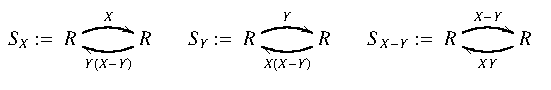
\includegraphics[width=0.73\textwidth]{figures/Fig_113_PDF209_Book197.pdf}
  \caption{$XY(X-Y)$ 的三个基本矩阵分解（原书 p.197）}
  \label{fig:three-line-matrix-factorizations}
\end{figure}
对每个 $Z\in\{X,Y,X-Y\}$，都有
\[
  \operatorname{End}_{\mathrm{MF}}(S_Z,S_Z)=\frac{\mathbb C[U]}{(U^2)},
\]
其中 $U$ 是乘积 $W/Z$ 中的一个因子。任取其中一个因子都可以，因为它们代表同一个上同调类，至多相差一个符号。

另一方面，$\operatorname{Sing}(W)$ 只有一个点 $p=0$。把 $W$ 写成 $X(XY)+Y(-XY)$，便得到矩阵分解
\[
\begin{aligned}
  M_p&\cong\left(R\oplus R\,dX\wedge dY\oplus R\,dX\oplus R\,dY,
  \begin{pmatrix}
    0&0&X&Y\\
    0&0&XY&XY\\
    XY&-Y&0&0\\
    -XY&X&0&0
  \end{pmatrix}\right)\\
  &\cong\left(R\oplus R\oplus R[1]\oplus R[1],
  \begin{pmatrix}
    0&0&X&Y\\
    0&0&0&X(X-Y)\\
    Y(X-Y)&-Y&0&0\\
    0&X&0&0
  \end{pmatrix}\right)\\
  &\cong\operatorname{Cone}\bigl(S_X\xrightarrow{Y}S_X[1]\bigr).
\end{aligned}
\]
因此 $M_p$ 由 $S_X$ 生成。另一方面，若 $\phi\colon M_p\to M_p$ 是次数为 $1$ 的态射，它来自复合
\[
  M_p\longrightarrow S_X\cong S_X[1]\longrightarrow M_p,
\]
则 $\operatorname{Cone}(\phi)\cong S_X\oplus S_X[1]$。因此 $M_p$ 分裂生成 $S_X$。类似推理表明，它也分裂生成 $S_Y,S_{X-Y}$，甚至生成整个范畴。
\end{example}

这些例子可以推广为三个重要定理。

\begin{theorem}{Knörrer 周期性\bookcite{140}}{knorrer-periodicity}
若 $W\in R=\mathbb C[X_1,\ldots,X_n]$，则
\[
  \mathrm{MF}^{\pm}(R,W)\cong_\infty
  \mathrm{MF}^{\pm}(R[U,V],W+UV).
\]
\end{theorem}

\begin{theorem}{Dyckerhoff 生成定理\bookcite{69}}{dyckerhoff-generation}
若 $W\in R=\mathbb C[X_1,\ldots,X_n]$ 只有一个孤立奇点，即 $\operatorname{Sing}(W)=\{p\}$，则 $\mathrm{MF}^{\pm}(R,W)$ 由 $M_p$ 分裂生成。
\end{theorem}

\begin{theorem}{Buchweitz 奇点范畴等价\bookcite{46}}{buchweitz-singularity-category}
矩阵分解范畴 $\mathrm{MF}^{0}(R,W)$ 等价于簇 $X=W^{-1}(0)$ 的奇点范畴\index{qidianfanchou@奇点范畴|hyperpage}，该范畴定义为商
\[
  \operatorname{Sing}X:=\frac{D^b\mathrm{Coh}\,X}{\mathrm{Perf}\,X}.
\]
\end{theorem}
这个等价把矩阵分解 $P$ 送到 $R/(W)$-模 $P_0/\operatorname{Im}d_1$，并将它视为 $X=V(R/(W))$ 上的层。

\begin{note}\label{note:matrix-factorization-category-equivalence}
\textbf{注 7.67.} 这个定理是用三角范畴而不是 $A_\infty$ 范畴表述的。若要把该等价理解为 $A_\infty$ 范畴之间的等价，可以使用 Drinfeld 商\bookcite{67}；此时矩阵分解范畴必须解释为 $2$-周期的 $\mathbb Z$-分次范畴，而非 $\mathbb Z_2$-分次范畴。
\end{note}

\begin{note}\label{note:singularity-category-kills-smooth-locus}
\textbf{注 7.68.} 奇点范畴 $\operatorname{Sing}X$ 之所以得名，是因为商构造会消去所有支撑在 $X$ 光滑部分上的层。这些层都有有限长度的局部自由分解，因此属于 $\mathrm{Perf}^{\bullet}X$。若 $X$ 是光滑簇，则 $\mathrm{Perf}^{\bullet}X=D\mathrm{Coh}^{\bullet}X$，所以相应商范畴为零。
\end{note}

矩阵分解的缺点是它把我们限制在 $\mathbb Z_2$-分次情形。可以通过使用分次代数来绕开这一限制。

\begin{definition}{分次 Landau--Ginzburg 模型}{graded-landau-ginzburg-model}\index{fencilandauginzburgmoxing@分次 Landau–Ginzburg 模型|hyperpage}
分次 Landau--Ginzburg 模型是二元组 $(R,W)$，其中 $R$ 是分次环，$W\in R$ 是次数为 $w$ 的齐次元。
\begin{itemize}
  \item $(R,W)$ 的分次矩阵分解\index{fencijuzhenfenjie@分次矩阵分解|hyperpage}是图表
  \[
    P=P_0\underset{d_1}{\overset{d_0}{\rightleftarrows}}P_1,
  \]
  其中 $P_0,P_1$ 是分次投射 $R$-模，$d_0,d_1$ 的次数分别为 $0,w$，并且
  \[
    d_1d_0=W1_{P_0},\qquad d_0d_1=W1_{P_1}.
  \]
  \begin{figure}[H]\centering
    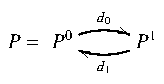
\includegraphics[width=0.30\textwidth]{figures/Fig_114_PDF210_Book198.pdf}
    \caption{分次矩阵分解（原书 p.198）}
    \label{fig:graded-matrix-factorization}
  \end{figure}
  \item 分次矩阵分解 $P$ 的同调移位为
  \[
    P[1]=P_1\underset{-d_0}{\overset{-d_1}{\rightleftarrows}}P_0(w).
  \]
  注意，$P[2]$ 与 $P(w)$ 相同，其中 $(w)$ 表示 $R$-分次的移位。
  \begin{figure}[H]\centering
    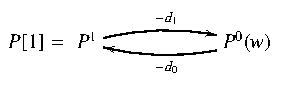
\includegraphics[width=0.34\textwidth]{figures/Fig_115_PDF210_Book198.pdf}
    \caption{矩阵分解的同调移位（原书 p.198）}
    \label{fig:graded-matrix-factorization-shift}
  \end{figure}
  \item 若 $P,Q$ 是两个分次矩阵分解，则定义
  \[
    \operatorname{Hom}^{\bullet}(P,Q)
    =\bigoplus_i\operatorname{grHom}_R(P_0,Q[i]_0)
      \oplus\operatorname{grHom}_R(P_1,Q[i]_1),
  \]
  其中 $\operatorname{grHom}_R(X,Y)$ 表示保持次数的 $R$-模态射。在这个空间上，标准微分关于同调分次的次数为 $1$。
  \item 分次矩阵分解范畴\index{fencijuzhenfenjiefanchou@分次矩阵分解范畴|hyperpage} $\mathrm{grMF}^{\bullet}(R,W)$ 是具有上述对象与态射的 dg-范畴的极小模型。
\end{itemize}
\end{definition}

\begin{example}[分次矩阵分解的不同实现]
回到 $R=\mathbb C[X,Y]$ 与 $W=XY(X-Y)$。把 $W$ 分解为 $X$ 与 $Y(X-Y)$，所得普通矩阵分解在忽略同调移位后，可以有三种不同的分次矩阵分解实现，如下图所示。
\begin{figure}[H]\centering
  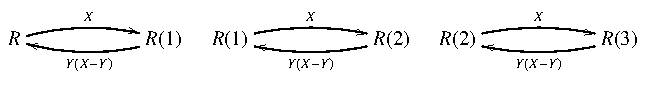
\includegraphics[width=0.92\textwidth]{figures/Fig_116_PDF211_Book199.pdf}
  \caption{例 7.70 中的三种分次矩阵分解（原书 p.199）}
  \label{fig:graded-factorization-three-gradings}
\end{figure}
\end{example}

分次矩阵分解的更多细节见 Orlov 的工作\bookcite{200}；其主要定理也将在下一节讨论。Landau--Ginzburg 模型还可以推广到非仿射\bookcite{201,225}或带栈结构\bookcite{216}的情形。此外，关于稳定表示范畴已有大量文献；它是奇点范畴的非交换类比\bookcite{46,108}。

\section{等价}\label{sec:equivalences}
\takeaway{Fano 与反 Fano 簇可由导出范畴借助 Serre 函子重构；Fourier--Mukai 核 $P\in D\mathrm{Coh}^{\bullet}(X\times Y)$ 给出函子 $\Phi_P=D\pi_{Y*}\circ(-\otimes P)\circ D\pi_X^*$，Orlov 定理说光滑射影簇间的正合函子皆源于此；模空间与倾斜把 $D\mathrm{Coh}^{\bullet}X$ 与箭图表示、$\mathrm{Perf}^{\bullet}A$ 联系起来。}
我们已经看到，$B$ 模型有许多不同形式，而不同的 $B$ 模型往往会导出等价或相关的范畴。本节将更深入地研究这一现象。

\subsection{重构簇}\label{subsec:reconstructing-varieties}
若 $A$ 是一个代数，则每个 $r\in Z(A)$ 都给出自然变换
\[
  \nu_r\colon 1_{\mathrm{Mod}A}\longrightarrow1_{\mathrm{Mod}A},
\]
它把模 $M$ 上对应于乘以 $r$ 的映射赋给 $M$。这确实是自然变换，因为 $r$ 的作用与所有模态射相容。反过来，任意从恒等函子到自身的自然变换都具有这种形式：令 $r=\nu_A(1)$。对任意模 $M$ 及元素 $m\in M$，定义模态射 $\phi_m\colon A\to M$，使 $\phi_m(1)=m$，则
\[
  \nu_M(m)=\nu_M(\phi_m(1))=\phi_m(\nu_A(1))=\phi_m(r)=rm.
\]
同样的论证也适用于包含 $A$ 本身的其他模范畴，例如 $\mathrm{Mod}A$、$D\mathrm{Mod}^{\bullet}A$ 和 $\mathrm{Perf}^{\bullet}A$。对仿射簇，这给出
\[
  \operatorname{End}(1_{D\mathrm{Coh}^{\bullet}X})
  \cong \operatorname{End}(1_{D\mathrm{Mod}^{\bullet}V(R)})\cong R.
\]
换言之，我们可以从仿射簇的导出范畴重构该簇：它就是
\[
  V\bigl(\operatorname{End}(1_{D\mathrm{Coh}^{\bullet}X})\bigr).
\]

对拟射影簇，这种方法通常行不通，因为它们的整体函数往往很少。此时，我们希望把簇写成某个分次环 $R$ 的 $\mathbb P(R)$。与仿射簇的坐标环不同，分次环 $R$ 并不能由 $X$ 唯一确定。取而代之的是，存在一个线丛 $L=\mathcal O(1)$，使
\[
  R=\bigoplus_{i\geq0}L^{\otimes i}(X).
\]

\begin{definition}{极丰富线丛与丰富线丛}{very-ample-ample-line-bundle}
若线丛 $L$ 满足 $X=\mathbb P(R_L)$，其中
\[
  R_L:=\bigoplus_{i\geq0}L^{\otimes i}(X),
\]
则称 $L$ 为极丰富线丛\index{jifengfuxiancong@极丰富线丛|hyperpage}；若存在 $k\geq1$ 使 $L^{\otimes k}$ 极丰富，则称 $L$ 为丰富线丛\index{fengfuxiancong@丰富线丛|hyperpage}。
\end{definition}

\begin{example}[射影直线上的丰富线丛]
一般而言，一个射影簇可以有许多丰富线丛。对 $\mathbb P^1$，所有 $\mathcal O(i)$（$i>0$）都是丰富的。以 $L=\mathcal O(2)$ 为例，则
\[
  R_L=\bigoplus_{i\geq0}\mathcal O(2i)(\mathbb P^1)
  =\mathbb C[X^2,Y^2,XY]
  \cong\frac{\mathbb C[U,V,W]}{(UV-W^2)}.
\]
由后一种描述可知，$\mathbb P(R_L)$ 可看作 $\mathbb P^2$ 中的圆锥曲线 $UV-W^2=0$。它通过 Veronese 嵌入
\[
  (x:y)\longmapsto(x^2:y^2:xy)
\]
与 $\mathbb P^1$ 同构。
\end{example}

从范畴角度看，我们可以把 $R_L$ 重构为自然变换空间。任一线丛都定义了 $\mathrm{Vect}(X)$ 上的自函子 $-\otimes L$：
\[
  (M\otimes L)(U):=M(U)\otimes_{\mathcal O(U)}L(U).
\]
这个函子在 $\mathrm{Vect}^{\bullet}(X)$ 上诱导 dg-函子，并在其导出范畴 $D\mathrm{Vect}^{\bullet}X=\mathrm{Perf}^{\bullet}X$ 上诱导一个 $A_\infty$ 函子 $T$（在导出范畴语境中，通常把它记为 $-\otimes^{\mathbf L}L$）。$L$ 的整体截面对应于恒等函子到 $T$ 的自然变换：
\[
  L(X)=\operatorname{Fun}(1,T).
\]
这里 $\operatorname{Fun}$ 表示从 $\mathrm{Perf}^{\bullet}X$ 到自身的函子范畴，其态射为自然变换。因为 $T$ 可逆，且 $T^{-1}=-\otimes L^{-1}$、$L^{-1}=\operatorname{Hom}(L,\mathcal O_X)$，故
\[
  \operatorname{Fun}(T^i,T^j)
  =\operatorname{Fun}(1,T^{j-i})
  =\operatorname{Fun}(1,-\otimes L^{j-i}).
\]
因此
\[
  R_T:=\bigoplus_{i\geq0}\operatorname{Fun}(1,T^i)
\]
通过复合获得环结构，并且与 $R_L$ 同构。于是，重构簇的问题归结为找到合适的 $T$。

如定义~\ref{def:tangent-cotangent-canonical-sheaves} 所述，簇上有一个内蕴地定义的线丛，即典范线丛。但是，它未必丰富，因此未必适合上述方法。为此，我们区分以下几类簇。

\begin{definition}{Fano 簇、Calabi--Yau 簇与反 Fano 簇}{fano-calabi-yau-antifano}
光滑射影簇 $X$ 称为：
\begin{itemize}
  \item 若反典范线丛 $K^{-1}$ 丰富，则称为 Fano 簇\index{fanocu@Fano 簇|hyperpage}；
  \item 若典范线丛平凡，即 $K=\mathcal O_X$，则称为 Calabi--Yau 簇\index{calabiyaucu@Calabi–Yau 簇|hyperpage}；
  \item 若典范线丛 $K$ 丰富，则称为反 Fano 簇\index{fanfanocu@反 Fano 簇|hyperpage}。
\end{itemize}
\end{definition}

\begin{note}\label{note:three-variety-types-curvature}
\textbf{注 7.74.} 这三种情形并未穷尽所有可能，但它们代表了三个基本类型，大致分别对应正曲率、零曲率和负曲率的流形。
\end{note}

\begin{example}[射影空间超曲面的分类]
射影空间 $\mathbb P^n$ 是 Fano 簇，因为 $K^{-1}=\mathcal O(n+1)$ 丰富。设 $f$ 是环 $R=\mathbb C[X_0,\ldots,X_n]$ 中次数为 $k$ 的齐次函数。由伴随公式\bookcite{109}，若 $\mathbb P(R/(f))$ 光滑，则当 $k<n+1$ 时它是 Fano 簇；当 $k=n+1$ 时它是 Calabi--Yau 簇；当 $k>n+1$ 时它是反 Fano 簇。

取 $n=2$，这也说明了前述曲率类比：当 $k=1,2$ 时，$\mathbb P(R/(f))$ 是 Fano 簇，即射影直线或二次曲线，因而同构于黎曼球面。当 $k=3$ 时所得簇是 Calabi--Yau 簇，即椭圆曲线；它是环面，故为平坦的。反 Fano 情形对应于亏格更高、具有负曲率的曲线。
\end{example}

这些讨论表明，如果光滑射影簇是 Fano 簇或一般型簇，我们或许可以从其导出范畴 $D\mathrm{Coh}^{\bullet}X=\mathrm{Perf}^{\bullet}X$ 重构它，因为此时可以尝试寻找函子 $-\otimes K$。

\begin{theorem}{Bondal--Orlov 重构定理}{bondal-orlov-reconstruction}
若 $X$ 是 Fano 簇或反 Fano 簇，则可以从 $D\mathrm{Coh}^{\bullet}X$ 重构 $X$。
\end{theorem}
\begin{proof}[证明思路]
证明的主要工具是 Serre 函子\index{serrehanzi@Serre 函子|hyperpage}。若 $\mathcal C$ 是 $k$-线性范畴，若存在函子 $F\colon\mathcal C\to\mathcal C$ 及自然同构
\[
  \nu_{X,Y}\colon\mathcal C(X,Y)\longrightarrow\mathcal C(Y,F(X))^\vee,
\]
其中 $(-)^\vee$ 表示 $k$-线性对偶，则称 $F$ 为 Serre 函子。若范畴有 Serre 函子，它在自然同构意义下唯一，因此是范畴的内在对象。$n$ 维光滑射影簇 $X$ 的导出范畴有 Serre 函子 $-\otimes K[n]$。当 $K$ 或 $K^{-1}$ 丰富时，Bondal 与 Orlov\bookcite{32}利用该 Serre 函子在导出范畴中识别点层\index{dianceng@点层|hyperpage}与线丛。
\end{proof}
% [Tutor Note: 原书把 Serre 函子的自然同构印作 $\nu_{X,Y}\colon\mathcal C(X,Y)\to\mathcal C(F(Y),X)^\vee$，这与紧接着所说的“$n$ 维光滑射影簇的导出范畴有 Serre 函子 $-\otimes K[n]$”不相容（按该书面公式，$-\otimes K[n]$ 满足的是关于 $F^{-1}$ 的关系）。译文采用标准方向 $\mathcal C(X,Y)\cong\mathcal C(Y,F(X))^\vee$；核对 Serre 对偶时可写成 $\operatorname{Hom}(X,Y)\cong\operatorname{Hom}(Y,X\otimes K[n])^\vee$，方向记反是最常见的错误。]

\subsection{Fourier--Mukai 变换}\label{subsec:fourier-mukai-transforms}
若簇不是 Fano 簇或一般型簇，则可能出现非同构簇却具有等价导出范畴的情形。为寻找这类现象的例子，我们先介绍一大类定义在相干层导出范畴之间的函子，再考察它们何时是等价。

这一构造的灵感来自 Fourier 分析。若 $f\colon\mathbb R\to\mathbb C$ 是函数，可以定义其 Fourier 变换
\[
  \mathcal F(f)\colon\mathbb R\to\mathbb C,
  \qquad y\longmapsto\int_{\mathbb R}f(x)e^{-ixy}\,dx.
\]
虽然这个运算把 $\mathbb R$ 上的函数变为 $\mathbb R$ 上的函数，但更好的看法是：它把一个空间 $X=\mathbb R$（位置空间）上的函数变成另一个空间 $Y$（动量空间）上的函数，只不过此处 $Y$ 恰好也同构于 $\mathbb R$。若把 $X$ 换成圆周 $S^1$，这一点就更明显：此时 $Y=\mathbb Z$，Fourier 变换把周期函数变成它的 Fourier 级数。

Fourier 变换具体如何作用？它先沿投影 $\pi_X\colon X\times Y\to X$ 把 $X$ 上的函数拉回到 $X\times Y$，再乘以 $X\times Y$ 上的一个函数，最后对 $X$ 分量积分消去。下面我们试着把这个过程从函数推广到层。

\begin{definition}{簇的笛卡尔积}{product-of-varieties}
若 $X,Y$ 是仿射簇，定义它们的笛卡尔积\index{dikaerji@笛卡尔积|hyperpage}为
\[
  X\times Y:=V(\mathcal O_X\otimes_{\mathbb C}\mathcal O_Y).
\]
若 $X,Y$ 是簇，分别有开覆盖 $\mathcal U=\{U_i:i\in I\}$ 和 $\mathcal V=\{V_j:j\in J\}$，则定义 $X\times Y$ 为由 $U_i\times V_j$ 覆盖、并配备显然粘合映射的簇。
\end{definition}

\begin{note}\label{note:product-topology-varieties}
\textbf{注 7.78.} 作为集合，$X\times Y$ 确实是 $X$ 与 $Y$ 的乘积；但就 Zariski 拓扑而言，它一般不是两个拓扑空间的乘积。此外可以证明，若 $X,Y$ 都光滑，则 $X\times Y$ 也光滑。
\end{note}

现在设 $X,Y$ 是光滑簇，且 $P^{\bullet}$ 是 $\mathrm{Perf}^{\bullet}(X\times Y)$ 中的对象。我们分三步构造一个函子。
\begin{enumerate}[label=(\roman*)]
  \item \textbf{提升到乘积空间。} 若 $M$ 是 $X$ 上的层，定义
  \[
    (\pi_X^*M)(U_i\times V_j):=M(U_i)\otimes_{\mathbb C}\mathcal O(V_j).
  \]
  若 $M$ 局部自由，则 $\pi_X^*M$ 也局部自由。因此这给出函子 $\pi_X^*\colon\mathrm{Vect}(X)\to\mathrm{Vect}(X\times Y)$，并进而给出 $A_\infty$ 函子
  \[
    D\pi_X^*\colon\mathrm{Perf}^{\bullet}(X)\to\mathrm{Perf}^{\bullet}(X\times Y).
  \]
  \item \textbf{与 $P^{\bullet}$ 张量。} 对簇 $V$ 上有限生成的局部自由层复形 $P^{\bullet}$（此处 $V=X\times Y$），可以定义层函子
  \[
    -\otimes P^{\bullet}\colon\mathrm{Vect}^{\bullet}V\longrightarrow\mathrm{Vect}^{\bullet}V,
    \qquad M^{\bullet}\longmapsto(M\otimes P)^{\bullet},
  \]
  其中
  \[
    (M\otimes P)^i(U)=\bigoplus_{k+\ell=i}M^k(U)\otimes P^{\ell}(U),
    \qquad d_{M\otimes P}=d_M\otimes1_P\pm1_M\otimes d_P.
  \]
  取 Čech 上同调后便得到 $A_\infty$ 函子
  \[
    D(-\otimes P)\colon\mathrm{Perf}^{\bullet}V\to\mathrm{Perf}^{\bullet}V.
  \]
  \item \textbf{对 $X$ 积分消去。} 若 $N$ 是 $X\times Y$ 上的层，我们希望令
  \[
    (\pi_{Y*}N)(V_j)=N(X\times V_j).
  \]
  但从 $A_\infty$ 的角度看，这个运算并不理想。事实上，$N(X\times V_j)$ 是层 $N(-\times V_j)\colon U_i\mapsto N(U_i\times V_j)$ 的零次 Čech 上同调；这种做法取了一个复形的同调，性质并不好。更好的办法是保留整个复形：
  \[
    (D\pi_{Y*}N)(V_j)=\check C\bigl(N(-\times V_j);\mathcal U\bigr).
  \]
  这样会把局部自由层变为局部自由层的复形。不过，这类复形未必有限生成，故得到的函子是
  \[
    D\pi_{Y*}\colon\mathrm{Perf}^{\bullet}(X\times Y)\to D\mathrm{VECT}^{\bullet}Y.
  \]
\end{enumerate}

\begin{note}\label{note:pushforward-perfect}
\textbf{注 7.79.} 一般而言，$N(U_i\times V_j)$ 不是有限生成的 $\mathcal O(V_j)$-模，所以这些 Čech 复形属于 $D\mathrm{VECT}^{\bullet}Y$，而非 $\mathrm{Perf}^{\bullet}Y$。不过，若 $X$ 是光滑射影簇，这些复形的上同调有限秩，因此 $D\pi_{Y*}$ 可以视为取值于 $\mathrm{Perf}^{\bullet}(Y)$ 的函子。
\end{note}

\begin{definition}{Fourier--Mukai 核与变换}{fourier-mukai-transform}
设 $X,Y$ 是光滑射影簇。Fourier--Mukai 核是对象 $F\in D\mathrm{Coh}^{\bullet}(X\times Y)$。把 $F$ 表示为 $X\times Y$ 上局部自由层组成的复形 $P^{\bullet}\in\mathrm{Vect}^{\bullet}(X\times Y)$，则相应的 Fourier--Mukai 变换\index{fouriermukaibianhuan@Fourier–Mukai 变换|hyperpage}是函子
\[
  \mathcal F_F:=D\pi_{Y*}\circ D(-\otimes P^{\bullet})\circ D\pi_X^*
  \colon\mathrm{Perf}^{\bullet}X\longrightarrow\mathrm{Perf}^{\bullet}Y.
\]
\end{definition}
% [Tutor Note: 合成顺序不可交换：$\Phi_P=D\pi_{Y*}\circ D(-\otimes P)\circ D\pi_X^*$ 是先沿 $\pi_X$ 拉回到 $X\times Y$、与核 $P$ 张量、再沿 $\pi_Y$ 推前，得到 $\mathrm{Perf}^{\bullet}X\to\mathrm{Perf}^{\bullet}Y$。核所在空间与函子方向的对应是：$P\in D\mathrm{Coh}^{\bullet}(X\times Y)$ 决定 $X\to Y$，把 $P$ 换成它在交换因子后的转置才给出反向函子；$p_2^*\mathcal E\otimes p_1^*(-)$ 的写法只是把拉回与张量换序的等价格式，不能据此调换 $X,Y$。]

\begin{example}[几种熟悉的函子]
Fourier--Mukai 变换的适用范围很广，能够描述一些熟知的函子。
\begin{itemize}
  \item 若 $Y$ 是一点，可以把结构层 $\mathcal O_X$ 看成 $X\times Y$ 上的层。对应的 Fourier--Mukai 变换把 $X$ 上的层 $S$ 送到它的 Čech 上同调，并将其视为 $\mathrm{Perf}^{\bullet}Y=\mathrm{vect}^{\bullet}_{\mathbb C}$ 中的对象。
  \item 令 $X=Y$，并考虑对角线的结构层
  \[
    \mathcal O_{\Delta}(U_i\times U_j)=\mathcal O_X(U_i\cap U_j).
  \]
  以 $\mathcal O_\Delta$ 为核的 Fourier--Mukai 变换同构于恒等函子。这类似于公式
  \[
    \int_{\mathbb R}f(y)\delta(x-y)\,dy=f(x),
  \]
  其中 $\delta$ 是 Dirac δ 函数。
  \item 若 $S$ 是 $X$ 上的可逆层，可以把它变成一个集中在对角线上的 $X\times X$ 上的层：
  \[
    S_\Delta(U_i\times U_j)=S_X(U_i\cap U_j).
  \]
  以 $S_\Delta$ 为核的 Fourier--Mukai 变换对应于与 $S$ 张量。
  \item 若 $\phi\colon X\to Y$ 是簇态射，则可构造其图像的结构层
  \[
    \mathcal O_\Gamma(U)=\frac{\mathcal O_{X\times Y}(U)}{(f\mid f(x,\phi(x))=0)}.
  \]
   以 $\mathcal O_\Gamma$ 为核的 Fourier--Mukai 变换对应于沿 $\phi$ 的导出推前。
\end{itemize}
在以上例子中，点层都被送到点层。不过，还有更精细的例子。
\end{example}

\begin{example}[椭圆曲线上的 Fourier--Mukai 等价]
考虑椭圆曲线 $E=\mathbb P(R)$，其中
\[
  R=\mathbb C[X,Y,Z]/(Y^2Z-X^3+XZ^2).
\]
对每个点 $P\in E$，都有一个线丛 $L_P=\mathcal O(P-P_\infty)$（参见例~\ref{ex:divisor-sheaf}）。为了区分椭圆曲线的两个副本——一个参数化点，另一个参数化线丛——把后者记作 $E^\vee$。

我们可以把这些线丛汇集为 $E^\vee\times E$ 上的一个大线丛 $T$，其在 $(P,Q)$ 处的纤维就是 $L_P$ 在 $Q$ 处的纤维。这个线丛称为 Poincaré 线丛。以它为核，可以定义从 $D\mathrm{Coh}^{\bullet}E^\vee$ 到 $D\mathrm{Coh}^{\bullet}E$ 的 Fourier--Mukai 变换；该变换把 $P$ 处的点层送到线丛 $L_P$。可以证明，这个函子实际上是一个等价。

Mukai\bookcite{183}把这一构造推广到高维，得到阿贝尔簇 $A$ 与其对偶簇 $A^\vee$ 之间的等价。这由此给出了不同簇之间导出等价的第一个例子。
\end{example}

本节最后介绍 Orlov 的一个漂亮定理：若限制在光滑射影簇上，Fourier--Mukai 构造足以描述簇之间所有相关的导出等价。

\begin{theorem}{Orlov 定理\bookcite{198}}{orlov-fourier-mukai}
光滑射影簇的导出范畴之间的每个正合函子，都同构于某个 Fourier--Mukai 变换。
\end{theorem}

Fourier--Mukai 变换的更多内容可参阅 Huybrechts 的专著\bookcite{124}。

\subsection{模空间}\label{subsec:moduli-spaces}
上一个例子中，我们使用了参数化 $D\mathrm{Coh}^{\bullet}E$ 中某些对象（次数为零的线丛）的空间 $E^\vee$。这个空间使我们能够把 $D\mathrm{Coh}^{\bullet}E$ 中的对象变换为 $D\mathrm{Coh}^{\bullet}E^\vee$ 中的对象。当然，这个想法并不局限于相干层的导出范畴，也可以用于其他范畴。

设 $A=\mathbb C Q/I$ 是带关系的箭图路径代数，并固定维数向量 $\alpha\colon Q_0\to\mathbb N$。定义表示空间
\[
  \operatorname{Rep}(Q,\alpha)
  :=\bigoplus_{a\in Q_1}\operatorname{Mat}_{\alpha_{h(a)}\times\alpha_{t(a)}}(\mathbb C),
\]
它可视为一个大仿射空间，其坐标环为
\[
  R=\mathbb C[X^a_{ij}\mid a\in Q_1,
       1\leq i\leq\alpha_{h(a)},\ 1\leq j\leq\alpha_{t(a)}].
\]
此空间中的每个点由一个 $|Q_1|$ 元组的矩阵 $(\rho_a)_{a\in Q_1}$ 表示，并对应一个表示 $\rho\colon\mathbb C Q\to\operatorname{Mat}_{n\times n}(\mathbb C)$，其中 $n=\sum_{v\in Q_0}\alpha_v$；对每条箭头 $a$，该表示把 $\rho_a$ 放入相应的分块矩阵中。我们可以把这些表示汇集成 $\operatorname{Rep}(Q,\alpha)$ 上的向量丛 $\operatorname{Rep}(Q,\alpha)\times\mathbb C^n$。在代数一侧，这对应于自由 $R$-模 $T=R\otimes\mathbb C^n$ 及模态射 $\rho\colon\mathbb C Q\to\operatorname{End}_R(T)$。

表示空间中的许多点对应同构的表示。为处理这一点，考虑换基群
\[
  \mathrm{GL}_\alpha:=\prod_{v\in Q_0}\mathrm{GL}_{\alpha_v}(\mathbb C),
\]
它在 $\operatorname{Rep}(Q,\alpha)$ 上的作用为
\[
  (g\cdot\rho)_a=g_{h(a)}\rho_a g^{-1}_{t(a)}.
\]
该作用的轨道恰好是表示的同构类。一个自然想法是取这个群作用的商\index{gitshang@GIT 商|hyperpage}，即考虑不变量环所对应的簇：
\[
  \operatorname{Rep}(Q,\alpha)//\mathrm{GL}_\alpha
  :=V(R^{\mathrm{GL}_\alpha}).
\]
与有限群的情形不同，这个商并不能参数化全部轨道。若群是无限的，一个轨道可能包含在另一个轨道的闭包中；此时每个不变量函数在这两个轨道上都取相同值，因此它们在商空间中对应同一点。

\begin{example}[Kronecker 箭图的商]
令 $Q$ 为下图所示的 Kronecker 箭图，并令 $\alpha=(1,1)$。于是 $\operatorname{Rep}(Q,\alpha)=\mathbb C^2$，$\mathrm{GL}_\alpha=(\mathbb C^*)^2$，且
\begin{figure}[H]\centering
  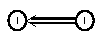
\includegraphics[width=0.20\textwidth]{figures/Fig_117_PDF218_Book206.pdf}
  \caption{例 7.84 中的箭图（原书 p.206）}
  \label{fig:kronecker-quiver-example-784}
\end{figure}
\[
  (g,h)\cdot(x,y)=(gxh^{-1},gyh^{-1}).
\]
该作用的轨道是去掉原点的直线 $\mathbb C(x,y)\setminus\{(0,0)\}$ 与零轨道 $\{(0,0)\}$；零轨道包含在所有其他轨道的闭包中。因此，范畴商只有一个点。事实上，坐标环为 $R=\mathbb C[X,Y]$，作用为
\[
  (g,h)\cdot X=gXh^{-1},\qquad(g,h)\cdot Y=gYh^{-1},
\]
所以 $R^{\mathrm{GL}_\alpha}=\mathbb C$，且 $\operatorname{Rep}(Q,\alpha)//\mathrm{GL}_\alpha=\{p\}$。

我们可以先丢弃不好的轨道，再取商。这样得到
\[
  \mathbb C^2\setminus\{(0,0)\}/\mathrm{GL}_\alpha=\mathbb P^1,
\]
这是一个射影簇，它分类除零表示外的所有轨道。这个商可以写作 $\mathbb P(R)$，其中 $R$ 按群作用分次：若 $f\in R$ 满足
\[
  (g,h)\cdot f=g^nh^{-n}f,
\]
就称 $f$ 的次数为 $n$。
\end{example}

上述例子可以推广为几何不变量理论（GIT）商。\footnote{GIT 是 geometric invariant theory（几何不变量理论）的缩写。}对每个向量 $\theta\colon Q_0\to\mathbb Z$，可构造乘法特征
\[
  \chi_\theta\colon\mathrm{GL}_\alpha\to\mathbb C^*,
  \qquad g\longmapsto\prod_{v\in Q_0}\det(g_v)^{\theta_v}.
\]
若 $f\in R$ 满足 $g\cdot f=\chi_\theta(g)f$，则称 $f$ 为 $\theta$-半不变量\index{banbubianliang@半不变量|hyperpage}。半不变量环\index{banbubianlianghuan@半不变量环|hyperpage}是各次幂 $\chi_\theta^n$ 对应半不变量空间的直和：
\[
  R_\theta:=\bigoplus_{n=0}^{\infty}
  \{f\in R\mid\text{对所有 }g\in\mathrm{GL}_\alpha,
  \ g\cdot f=\chi_\theta(g)^nf\}.
\]
这是一个分次环，其零次部分为不变量环 $R^{\mathrm{GL}_\alpha}$。簇 $\mathbb P(R_\theta)$ 可由开集
\[
  U_f=V\bigl((R_\theta[f^{-1}])_0\bigr),\qquad f\in(R_\theta)_n,
\]
覆盖。环 $R_\theta[f^{-1}]_0$ 的元素可看作定义在
$\{\rho\in\operatorname{Rep}(Q,\alpha)\mid f(\rho)\ne0\}$ 上的不变量函数，因此
\[
  U_f=\{\rho\in\operatorname{Rep}(Q,\alpha)\mid f(\rho)\ne0\}//\mathrm{GL}_\alpha.
\]

\begin{definition}{$\theta$-半稳定表示及其模空间}{theta-semistable-moduli}
若存在 $f\in(R_\theta)_{>0}$ 使 $f(\rho)\ne0$，则称表示 $\rho$ 为 $\theta$-半稳定表示\index{banwendingbiaoshi@半稳定表示|hyperpage}\index{wendingbiaoshi@稳定表示|hyperpage}。$\theta$-半稳定表示的模空间定义为
\[
  M_\theta(Q,\alpha):=\mathbb P(R_\theta),
\]
也可解释为
\[
  \operatorname{Rep}^{\theta\text{-ss}}(Q,\alpha)//\mathrm{GL}_\alpha
  :=\{\rho\in\operatorname{Rep}(Q,\alpha)\mid\rho\text{ 为 }\theta\text{-半稳定表示}\}//\mathrm{GL}_\alpha.
\]
\end{definition}

一般而言，两个不同构的 $\theta$-半稳定表示仍可能对应 $M_\theta(Q,\alpha)$ 中的同一点。这会在轨道大小不同时发生，因为较小的轨道可能包含在较大轨道的闭包中。最大的轨道对应于稳定子尽可能小的表示；最小稳定子就是标量矩阵群 $\mathbb C^*\subset\mathrm{GL}_\alpha$。因此，若一个半稳定表示的稳定子恰为 $\mathbb C^*$，就称它为 $\theta$-稳定表示。

(半)稳定性的定义来自 $\mathrm{GL}_\alpha$ 在簇 $\operatorname{Rep}(Q,\alpha)$ 上的群作用，但它也有一个漂亮的箭图表示论解释。

\begin{theorem}{King 稳定性判据}{king-stability-criterion}
表示 $\rho\in\operatorname{Rep}(Q,\alpha)$ 是 $\theta$-稳定的（$\theta$-半稳定的），当且仅当 $\theta\cdot\alpha=0$，且对每个真子表示，其维数向量 $\beta$ 都满足 $\theta\cdot\beta>0$（$\theta\cdot\beta\geq0$）。
\end{theorem}
\begin{proof}[证明思路]
这里只说明这种联系的主要思路，完整细节参见\bookcite{138}。首先，非零 $n\theta$-半不变量的存在蕴含 $\theta\cdot\alpha=0$，因为标量矩阵 $\lambda 1$ 对 $\rho$ 的作用平凡：
\[
  f(\rho)=f(\lambda1\cdot\rho)=\chi_\theta(\lambda1)^n f(\rho)
  =\lambda^{n\theta\cdot\alpha}f(\rho).
\]
若表示 $\rho$ 有维数向量为 $\beta$ 的子表示，就可将它写成分块上三角形式。用
\[
  g_t=\begin{pmatrix}t1_\beta&0\\0&1_{\alpha-\beta}\end{pmatrix}
\]
作共轭。由于表示具有上述分块上三角形式，极限 $\lim_{t\to0}g_t\cdot\rho$ 存在。但若 $f$ 是 $n\theta$-半不变量，则
\[
  f(g_t\cdot\rho)=t^{n\theta\cdot\beta}f(\rho).
\]
若 $\theta\cdot\beta<0$，当 $t\to0$ 时右侧没有极限，这就产生矛盾。
\end{proof}

\begin{definition}{泛型稳定条件}{generic-stability-condition}
若 $\theta\cdot\alpha=0$ 且对每个非零维数向量 $\beta<\alpha$ 都有 $\theta\cdot\beta\ne0$，则称稳定条件\index{fanxingwendingtiaojian@泛型稳定条件|hyperpage} $\theta$ 关于 $\alpha$ 是泛型的。这意味着 $\theta$-半稳定与 $\theta$-稳定两种概念一致。
\end{definition}

\begin{theorem}{King 模空间光滑性定理\bookcite{138}}{king-moduli-smoothness}
若 $\theta$ 是泛型的，则 $M_\theta(Q,\alpha)$ 是光滑簇，其点对应于 $Q$ 的 $\theta$-稳定 $\alpha$ 维表示的同构类。
\end{theorem}
\begin{proof}[证明思路]
空间 $\operatorname{Rep}^{\theta\text{-ss}}(Q,\alpha)$ 是光滑空间 $\operatorname{Rep}(Q,\alpha)$ 的开子集，故自身光滑。投影
\[
  \pi\colon\operatorname{Rep}^{\theta\text{-ss}}(Q,\alpha)
  \longrightarrow M_\theta(Q,\alpha)
\]
的纤维都同构于光滑簇 $\mathrm{GL}_\alpha/\mathbb C^*$，因而目标空间也必为光滑簇。
\end{proof}

\begin{example}[Kronecker 箭图表示的稳定模空间]
回到维数向量为 $\alpha=(1,1)$ 的 Kronecker 箭图。根据 $\theta=(\theta_1,\theta_2)$ 的不同取值，情况如下：
\begin{itemize}
  \item 若 $\theta_1+\theta_2\ne0$，则不存在 $\theta$-半不变量，故 $R_\theta=\mathbb C$、$\mathbb P(R_\theta)=\varnothing$。由于 $\alpha\cdot\theta\ne0$，不存在 $\theta$-半稳定表示，所以 $M_\theta(Q,\alpha)=\varnothing$。
  \item 若 $\theta_1=-\theta_2=0$，常数函数是 $\theta$-半不变量，故 $R_\theta=\mathbb C\oplus\mathbb C\oplus\cdots$，且 $\mathbb P(R_\theta)=\{p\}$。注意，此时 $\theta$ 不是泛型条件。所有表示都半稳定，但没有稳定表示。每个轨道的闭包都包含零轨道，因此 $M_\theta(Q,\alpha)$ 只有一个点。
  \item 若 $\theta_1=-\theta_2=k>0$，次数为 $k$ 的函数是 $\theta$-半不变量，故
  $R_\theta=\mathbb C\oplus R_k\oplus R_{2k}\oplus\cdots$，并且 $\mathbb P(R_\theta)=\mathbb P^1$。此时除零轨道外，所有表示都稳定；零轨道有维数向量 $(0,1)$ 的子表示。
  \item 若 $\theta_1=-\theta_2=k<0$，不存在 $\theta$-半不变量，故 $R_\theta=\mathbb C$ 且 $\mathbb P(R_\theta)=\varnothing$。此时没有稳定表示，因为每个表示都有维数向量 $(1,0)$ 的子表示。
\end{itemize}

若 $\theta$ 泛型，我们便能按同构分类所有 $\theta$-稳定表示。每个这样的表示都可视为一个带有 $\mathbb C Q$ 作用的向量空间 $\mathbb C^n$。自然的问题是：能否把这些表示组成 $M_\theta(Q,\alpha)$ 上的向量丛？朴素做法是考虑丛 $\operatorname{Rep}(Q,\alpha)\times\mathbb C^n\to\operatorname{Rep}(Q,\alpha)$，限制到稳定表示子空间后再对 $\mathrm{GL}_\alpha$ 取商。不幸的是，这样做行不通，因为每个点 $(\rho,x)$ 的轨道中都有 $(\rho,\lambda x)$（回忆标量 $\lambda\in\mathrm{GL}_\alpha$ 对 $\rho$ 的作用平凡）。于是 $(\rho,0)$ 落在所有 $(\rho,x)$ 的轨道闭包中，商仍只是 $M_\theta(Q,\alpha)$。

为避免这种情况，假设存在群态射 $\sigma\colon\mathrm{GL}_\alpha\to\mathbb C^*$，使其在 $\mathbb C^*\subset\mathrm{GL}_\alpha$ 上满足 $\sigma(\lambda)=\lambda$。把 $\mathrm{GL}_\alpha$ 在向量丛上的作用改为
\[
  g(\rho,x):=(g\cdot\rho,\sigma(g)^{-1}gx).
\]
这样标量在 $x$ 上的作用变为平凡，因而可对 $\operatorname{Rep}^{\theta\text{-ss}}(Q,\alpha)\times\mathbb C^n$ 取这个新作用的商。所得商称为泛丛；它可以视为 $M_\theta(Q,\alpha)$ 上的 $\mathbb C Q$-模层。
\end{example}

与交换情形类似，Fourier--Mukai 核可视为 $X$ 上的、以 $Y$ 上层为纤维的层；泛丛则是 $M_\theta(Q,\alpha)$ 上的、以与非交换代数 $\mathbb C Q$ 对应的非交换簇上的层为纤维的层。由此可定义非交换 Fourier--Mukai 变换
\[
  F\colon D\mathrm{Coh}^{\bullet}M_\theta(Q,\alpha)
  \longrightarrow D\mathrm{Mod}^{\bullet}\mathbb C Q.
\]

\begin{example}[Kronecker 模空间上的泛丛]
回到 $\alpha=(1,1)$、$\theta=(1,-1)$ 的 Kronecker 箭图，取 $\sigma(g,h)=h$。在
\[
  T=\mathbb C[X,Y]\otimes\mathbb C^2
  =\mathbb C[X,Y]e_1\oplus\mathbb C[X,Y]e_2
\]
上，$\mathrm{GL}_\alpha$ 的作用为
\[
  (g,h)e_1=h^{-1}ge_1,\qquad
  (g,h)e_2=h^{-1}he_2=e_2.
\]
因此，在 $M_\theta(Q,\alpha)=\mathbb P^1$ 上的重言丛为 $\mathcal O(1)\oplus\mathcal O$。

要计算 $\mathcal O(k)\in\mathrm{Perf}^{\bullet}\mathbb P^1$ 在 Fourier--Mukai 变换下的像，将它与 $T_\theta$ 张量，得到 $\mathcal O(k+1)\oplus\mathcal O(k)$。这个丛的 Čech 复形是一个无限维的分次 $\mathbb C Q$-表示。其底层两项复形为
\[
  \mathbb C[X]\oplus\mathbb C[X^{-1}]
  \xrightarrow{\ (1\quad X^k)\ }
  \mathbb C[X,X^{-1}],
  \qquad
  \mathbb C[X]\oplus\mathbb C[X^{-1}]
  \xrightarrow{\ (1\quad X^{k+1})\ }
  \mathbb C[X,X^{-1}],
\]
分别对应两项线丛的局部截面空间；图中竖直箭头给出 Kronecker 箭头在这些空间上的作用。\begin{figure}[H]\centering
  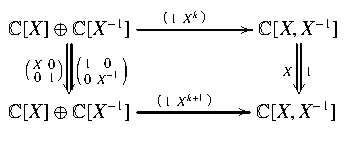
\includegraphics[width=0.90\textwidth]{figures/Fig_118_PDF221_Book209.pdf}
  \caption{例 7.90 中的 Čech 复形及箭图作用（原书 p.209）}
  \label{fig:cech-complex-tautological-bundle}
\end{figure}
水平映射是 Čech 复形的微分，竖直映射表示箭图箭头的作用。对该复形取上同调：若 $k\geq-1$，上同调集中在次数 $0$，得到表示
\[
  \mathbb C^{k+2}\xleftarrow{\left(\begin{smallmatrix}1_k\\)}\mathbb C^{k+1},
  \qquad
  \mathbb C^{k+2}\xleftarrow{\left(\begin{smallmatrix}0\\)}\mathbb C^{k+1}.
\]
若 $k<-1$，上同调集中在次数 $1$，得到表示
\[
  \mathbb C^{-k-1}\xleftarrow{\left(\begin{smallmatrix}1_k&0\end{smallmatrix}\right)}\mathbb C^{-k},
  \qquad
  \mathbb C^{-k-1}\xleftarrow{\left(\begin{smallmatrix}0&1_k\end{smallmatrix}\right)}\mathbb C^{-k}.
\]
\end{example}

\begin{note}\label{note:quiver-relations-moduli}
\textbf{注 7.91.} 模空间的构造也适用于带关系路径代数 $A=\mathbb C Q/I$。此时需要考虑子簇
\[
  \operatorname{Rep}(A,\alpha)
  =\{\rho\in\operatorname{Rep}(Q,\alpha)\mid\rho(I)=0\},
\]
或其某个不可约分支。该分支的坐标环 $R_A$ 是 $R$ 对一个 $\mathrm{GL}_\alpha$-不变理想 $i$ 取商所得。若此分支光滑且 $\theta$ 泛型，则
\[
  M_\theta(Q,\alpha)=\mathbb P\bigl(R_\theta/(i\cap R_\theta)\bigr)
\]
是光滑簇，并带有一个局部自由层，其纤维是 $\theta$-稳定的 $A$-模。由此可以构造 Fourier--Mukai 函子，但要判定该函子何时为等价并不容易。
\end{note}

\subsection{倾斜}\label{subsec:tilting}
非交换 Fourier--Mukai 变换与构造等价的另一种方法——倾斜——密切相关。

\begin{definition}{倾斜对象}{tilting-object}
设 $\mathcal C^{\bullet}$ 是一个极小且分裂闭的 $A_\infty$ 范畴。若对象 $T$ 是分裂生成元，且 $\mathcal C^{\bullet}(T,T)$ 集中在次数 $0$，则称 $T$ 为倾斜对象\index{qingxieduixiang@倾斜对象|hyperpage}。
\end{definition}

若 $T$ 是倾斜对象，则 $A=\mathcal C^{\bullet}(T,T)$ 是普通代数，因为次数原因，所有高阶乘积都为零。此外，
\[
  \mathcal C^{\bullet}\cong_\infty D^{\pi}A^{\bullet}
  \cong_\infty\mathrm{Perf}^{\bullet}A,
\]
所以所有对象都同构于有限生成投射 $A$-模所组成的有限复形。

若 $\mathcal C^{\bullet}$ 是 dg-范畴 $\mathrm{dg}\mathcal C^{\bullet}$ 的极小模型，且 $A=\mathrm{dg}\mathcal C^{\bullet}(T,T)$，则可以显式构造这些复形。对 $\mathrm{dg}\mathcal C^{\bullet}$ 中任意 $M$，复形 $\mathcal C^{\bullet}(M,T)$ 具有右 $A$-模结构，并且
\[
  d(ma)=(dm)a\pm m(da)=(dm)a,
\]
所以它实际上是右 $A$-模复形。映射
\[
  \operatorname{Hom}(-,T)\colon\mathrm{dg}\mathcal C^{\bullet}
  \longrightarrow\mathrm{TwMOD}^{\bullet}A,
  \qquad M\longmapsto\mathrm{dg}\mathcal C^{\bullet}(M,T)
\]
是一个 dg-函子。转到极小模型后，它给出 $A_\infty$ 函子
\[
  D\operatorname{Hom}(-,T)\colon\mathcal C^{\bullet}
  \longrightarrow D\mathrm{MOD}^{\bullet}A.
\]
由于 $T$ 的像是 $A$ 作为自身右模，且 $T$ 是分裂生成元，函子 $D\pi\operatorname{Hom}(-,T)$ 会把 $\mathcal C^{\bullet}$ 嵌入 $D\mathrm{MOD}^{\bullet}A$，其像是一个与 $\mathrm{Perf}^{\bullet}A$ 等价的全子范畴。

在特殊情形 $\mathrm{dg}\mathcal C^{\bullet}=\mathrm{Vect}^{\bullet}X$ 且 $T$ 是向量丛（即倾斜丛\index{qingxiecong@倾斜丛|hyperpage}）时，我们得到从 $\mathrm{Perf}^{\bullet}X$ 到 $\mathrm{Perf}^{\bullet}A$ 的函子，其中
\[
  A=\operatorname{Hom}(T,T)(X).
\]
该函子把一个向量丛复形与 $T$ 作层态射，随后取 Čech 上同调。但取层态射可以解释为与 $A$ 张量，其核是对偶层
\[
  T^\vee(U):=\operatorname{Hom}(T(U),\mathbb C),
\]
它是左 $A$-模层。因此，倾斜函子实际上是一个以 $T^\vee(U)$ 为核的非交换 Fourier--Mukai 变换。

\begin{example}[射影空间上的 Beilinson 倾斜丛]
射影直线 $\mathbb P^1$ 有倾斜丛 $\mathcal O\oplus\mathcal O(1)$；更一般地，$\mathbb P^k$ 有倾斜丛
\[
  \mathcal O\oplus\cdots\oplus\mathcal O(k).
\]
相应的自同态代数是如下箭图的路径代数：顶点为 $0,1,\ldots,k$，相邻顶点间有 $k+1$ 条箭头，记为 $a_i^u$（$0\leq u\leq k$）；其关系为
\[
  a_{i+1}^u a_i^v=a_{i+1}^v a_i^u.
\]
\begin{figure}[H]\centering
  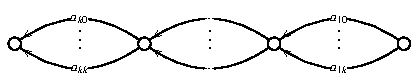
\includegraphics[width=0.92\textwidth]{figures/Fig_119_PDF222_Book210.pdf}
  \caption{$\mathbb P^k$ 上倾斜丛的箭图（原书 p.210）}
  \label{fig:tilting-projective-space-quiver}
\end{figure}
\end{example}

\begin{example}[带关系路径代数之间的倾斜]
不同的带关系路径代数也可以通过倾斜联系起来。最简单的例子是下图中的两个带关系箭图；后一个箭图是对象
\[
  T=S_2\oplus S_{23}\oplus P_2
\]
的自同态环（采用第\ref{subsec:linear-quiver}节所用记号）。
\begin{figure}[H]\centering
  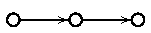
\includegraphics[width=0.31\textwidth]{figures/Fig_120_PDF223_Book211.pdf}\qquad
  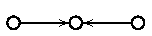
\includegraphics[width=0.31\textwidth]{figures/Fig_121_PDF223_Book211.pdf}
  \caption{倾斜前后的两个箭图（原书 p.211）}
  \label{fig:tilting-quiver-example}
\end{figure}
有限维代数的倾斜理论，更多内容参见\bookcite{10}。
\end{example}

\begin{note}\label{note:rarity-of-tilting-bundles}
\textbf{注 7.95.} 射影簇的相干层导出范畴有倾斜丛的情形相当少见。在一维时，只有射影直线有倾斜丛，其他曲线都没有；在二维时，有理曲面有倾斜丛\bookcite{120}。一般可以证明，若一个簇存在倾斜丛，则其 Grothendieck 群（见第\ref{ch:stability}章）是有限秩自由阿贝尔群。特别地，这排除了所有射影 Calabi--Yau 簇。
\end{note}

\subsection{矩阵分解与射影簇}\label{subsec:matrix-factorizations-projective-varieties}
设 $R=\mathbb C[X_0,\ldots,X_n]$，且 $f\in R$ 是次数为 $k$ 的齐次多项式。此时可以考虑两个范畴：
\begin{itemize}
  \item $X=\mathbb P(R/(f))$ 上相干层的导出范畴 $D\mathrm{Coh}^{\bullet}X$；
  \item 分次矩阵分解范畴 $\mathrm{grMF}^{\bullet}(R,f)$。
\end{itemize}
一般而言，这两个范畴并不等价，但彼此密切相关。

\begin{example}[三个齐次多项式的矩阵分解范畴]
考虑 $n=1$ 与三个函数
\[
  f_1=X,\qquad f_2=XY,\qquad f_3=XY(X-Y).
\]
簇 $X=\mathbb P(R/(f_k))$ 由 $k$ 个 $\mathbb P^1$ 上的点组成，且
\[
  X\subset\{(0:1),(1:0),(1:1)\}.
\]
因此 $X\cong V(\mathbb C^k)$，从而
\[
  D^b\mathrm{Coh}\,X\cong D^b\mathrm{mod}\,\mathbb C^k
  \cong D^b\mathrm{mod}\,\mathbb C Q,
\]
其中 $Q$ 是有 $k$ 个顶点且没有箭头的箭图。
\begin{itemize}
  \item 对 $f_1$，分次矩阵分解范畴是平凡的，因为 $V(R/(f_1))$ 是一条没有奇点的仿射直线。
  \item 对 $f_2$，范畴由下图所示的对象生成：
  \begin{figure}[H]\centering
    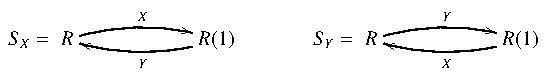
\includegraphics[width=0.78\textwidth]{figures/Fig_122_PDF223_Book211.pdf}
    \caption{$S_X$ 与 $S_Y$ 的矩阵分解（原书 p.211）}
    \label{fig:two-linear-matrix-factorizations}
  \end{figure}
  $S_X$ 与 $S_Y$ 的自同态环都同构于 $\mathbb C$，二者之间没有态射。因此
  \[
    \mathrm{grMF}^{\bullet}(R,f_2)\cong_\infty D\mathrm{mod}^{\bullet}\mathbb C Q,
  \]
  其中 $Q$ 是两个顶点且无箭头的箭图。
  \item 对 $f_3$，范畴由 $S_X(i),S_Y(i),S_{X-Y}(i)$ 生成。考察
  $S_X\oplus S_Y\oplus S_{X-Y}$ 的自同态代数，可见它同构于 $\mathbb C^3$。因此，这三个对象生成的子范畴与
  \[
    D\mathrm{mod}^{\bullet}\mathbb C^3
    \cong_\infty D\mathrm{Coh}^{\bullet}X
  \]
   等价；但这个子范畴并不等价于 $\mathrm{grMF}^{\bullet}(R,f_3)$。
% [Tutor Note: 原书此条（p.212）有两处把 $f_3$ 印成了 $f_2$：一是“$\mathrm{grMF}^{\bullet}(R,f_2)$ 中与 $D\mathrm{Coh}^{\bullet}X$ 等价的子范畴”，二是“不等价于 $\mathrm{grMF}^{\bullet}(R,f_2)$”。按上下文（本条讨论 $f_3=XY(X-Y)$，$f_2$ 的情形已在上一条处理）应为 $f_3$；译文已改。]
\end{itemize}
\end{example}

函数次数不同所导致的差异可以推广到所有射影空间的超曲面。

\begin{theorem}{Orlov 定理}{orlov-hypersurface}
设 $X=\mathbb P(R/(f))$ 是 $\mathbb P^n=\mathbb P(R)$ 中的光滑子簇，且 $k=\deg f$。则有以下函子：
\begin{enumerate}[label=(\roman*)]
  \item 若 $k<n+1$，则存在全忠实嵌入 $F\colon\mathrm{grMF}^{0}(R,f)\to D^b\mathrm{Coh}\,X$；
  \item 若 $k=n+1$，则存在等价 $F\colon D^b\mathrm{Coh}\,X\to\mathrm{grMF}^{0}(R,f)$；
  \item 若 $k>n+1$，则存在全忠实嵌入 $F\colon D^b\mathrm{Coh}\,X\to\mathrm{grMF}^{0}(R,f)$。
\end{enumerate}
\end{theorem}
\begin{proof}[证明思路]
涉及的两个范畴都可以构造为一个较大范畴的商：
\[
  D^b\mathrm{Coh}\,X\cong
  \frac{D^b\mathrm{grMod}\,R}{\langle\mathrm{grmod}\,R\rangle},
  \qquad
  \mathrm{grMF}^{0}(R,f)\cong
  \frac{D^b\mathrm{grMod}\,R}{\langle\mathrm{grProj}\,R\rangle}.
\]
两个分母分别是由有限维分次模和分次投射模生成的子范畴。在\bookcite{200}中，作者通过考察这两个子范畴在 $D^b\mathrm{grMod}\,R$ 中的相对位置，得到上述结论。

当 $k=n+1$ 时，Segal 与 Shipman\bookcite{216,225}还给出了一个漂亮的几何证明。把 $R$ 上的分次重新解释为群作用后，可以把 $\mathrm{grMF}(R,f)$ 看作商栈 $[\mathbb A^{n+1}/\mathbb Z_{n+1}]$ 上的矩阵分解范畴 $\mathrm{MF}([\mathbb A^{n+1}/\mathbb Z_{n+1}],f)$。这个栈与 $Y=|K_{\mathbb P^n}|$ 的典范丛全空间导出等价，因此可转而考察 $\mathrm{MF}(Y,f)$。在 $Y$ 上，$f$ 的零点由两部分组成：一部分是位于 $\mathbb P^n\subset |K_{\mathbb P^n}|=Y$ 中、在 $\mathbb P^n$ 上 $f$ 的零点之上的纤维，另一部分是 $\mathbb P^n$ 本身。因此奇点集为
\[
  X\subset\mathbb P^n\subset K_{\mathbb P^n}.
\]
局部而言，这是一个正规交，于是可用 Knörrer 周期性得到
\[
  \mathrm{MF}(Y,f)\simeq\mathrm{MF}(X,0)\cong D^b\mathrm{Coh}\,X.
\]
\end{proof}

\section{练习}\label{sec:exercises-chapter-seven}

\begin{exercise}\label{exer:varieties-same-finite-points}
设 $X_1,X_2$ 是两个仿射簇。
\begin{enumerate}[label=(\roman*)]
  \item 证明：若 $X_1,X_2$ 含有相同有限个点，则它们同构。
  \item 证明：若 $\mathrm{Coh}\,X_1\simeq\mathrm{Coh}\,X_2$，则 $X_1,X_2$ 同构（使用 Morita 等价）。
  \item 证明：对任意簇 $X$，有
  \[
    \mathcal O(X)\cong\operatorname{End}(1_{\mathrm{Perf}^{\bullet}X})
    \cong\operatorname{End}(1_{D\mathrm{Coh}^{\bullet}X}).
  \]
\end{enumerate}
\end{exercise}

\begin{exercise}\label{exer:product-varieties}
设 $X_1,X_2$ 是两个簇，分别有仿射开覆盖 $(U_{1,i})_i,(U_{2,j})_j$。把 $X_1\times X_2$ 看作由开集 $U_{1,i}\times U_{2,j}$ 覆盖的簇。
\begin{enumerate}[label=(\roman*)]
  \item 证明：若 $X_1=\mathbb P^n$、$X_2=\mathbb P^m$，则 $X_1\times X_2$ 可写成 $\mathbb P(R)$，其中 $R$ 是 $\mathbb C[X_0,\ldots,X_n,Y_0,\ldots,Y_m]$ 中由单项式 $X_iY_j$ 生成的子环。
  \item 令
  \[
    R=\mathbb C[X_1,\ldots,X_4]/(X_1^2+\cdots+X_4^2),\qquad \deg X_i=1.
  \]
  证明 $\mathbb P(R)$ 与 $\mathbb P^1\times\mathbb P^1$ 同构。
  \item 若 $M_1,M_2$ 分别是 $X_1,X_2$ 上的层，可在 $X_1\times X_2$ 上定义 $M_1\otimes M_2$，要求
  \[
    (M_1\otimes M_2)(U_{1,i}\times U_{2,j})
    =M_1(U_{1,i})\otimes M_2(U_{2,j}).
  \]
  证明：若 $M_1,M_2$ 局部自由，则 $M_1\otimes M_2$ 也局部自由。
\end{enumerate}
\end{exercise}

\begin{exercise}\label{exer:elliptic-curve-cohomology-and-generators}
令 $E=\mathbb P(R)$，其中
\[
  R=\mathbb C[X,Y,Z]/\bigl(Y^2Z-(X-\lambda_1Z)(X-\lambda_2Z)(X-\lambda_3Z)\bigr).
\]
\begin{enumerate}[label=(\roman*)]
  \item 证明 $E$ 光滑当且仅当 $\lambda_i$ 两两不同。以下各问均假设这一条件成立。
  \item 证明结构层的层上同调为 $\mathbb C\oplus\mathbb C$，分别集中在次数 $0,1$。
  \item 令 $S_p$ 是点 $p=(x:y:z)\in E$ 处的点层，构造它的局部自由分解。
  \item 利用该分解，计算 $D\mathrm{Coh}^{\bullet}E$ 中 $\mathcal O\oplus S_p$ 的自同态代数。证明该代数同构于下图箭图的路径代数模关系理想，其中关系为
  \begin{figure}[H]\centering
    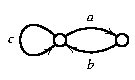
\includegraphics[width=0.27\textwidth]{figures/Fig_123_PDF225_Book213.pdf}
    \caption{练习 7.3(iv) 中的箭图（原书 p.213）}
    \label{fig:exercise-elliptic-endomorphism-quiver}
  \end{figure}
  \[
    \mathbb C Q/\langle ba,c^2\rangle.
  \]
  \item 可以证明 $\mathcal O$ 与 $S_p$ 分裂生成导出范畴。解释为什么这意味着 $\operatorname{End}(\mathcal O\oplus S_p)$ 上的 $A_\infty$ 结构必定非平凡。
\end{enumerate}
\end{exercise}

\begin{exercise}\label{exer:projective-hypersurface-smoothness}
令 $R=\mathbb C[X_0,\ldots,X_n]/(f)$，其中 $f$ 是次数为 $d$ 的不可约齐次函数。
\begin{enumerate}[label=(\roman*)]
  \item 证明 $V(R)$ 光滑当且仅当 $f$ 是线性的；此时 $V(R)\cong\mathbb A^n$。
  \item 证明：当 $d>1$ 时，对一般的 $f$，$\mathbb P(R)$ 光滑（也就是说，在所有次数为 $d$ 的齐次多项式组成的空间 $\mathbb C[X_0,\ldots,X_n]_d$ 中，光滑性构成一个稠密开条件）。
  \item 若 $\mathbb P(R)$ 光滑，证明 $K\cong\mathcal O(d-n-1)$；因此若 $d=n+1$，则 $\mathbb P(R)$ 是 Calabi--Yau 簇。
\end{enumerate}
\end{exercise}

\begin{exercise}\label{exer:quadric-surface-tilting}
令 $X=\mathbb P(R)$，其中
\[
  R=\mathbb C[X,Y,U,V]/(XY-UV),
\]
所有变量的次数均为 $1$。
\begin{enumerate}[label=(\roman*)]
  \item 求 $\mathrm{Perf}^{\bullet}X$ 中 $\mathcal O(0)\oplus\mathcal O(1)\oplus\mathcal O(2)\oplus\mathcal O(3)$ 的自同态环，并画出其箭图。
  \item 将 $X$ 识别为 $\mathbb P^1\times\mathbb P^1$。对每个 $(i,j)\in\mathbb Z^2$，定义
  \[
    \mathcal O(i,j)=\mathcal O_{\mathbb P^1}(i)\otimes\mathcal O_{\mathbb P^1}(j).
  \]
  求 $\mathcal O(0,0)\oplus\mathcal O(1,0)\oplus\mathcal O(0,1)\oplus\mathcal O(1,1)$ 的自同态环，并画出其箭图。
\end{enumerate}
\end{exercise}

\begin{exercise}\label{exer:matrix-factorizations-univariate}
令
\[
  f(X)=(X-\lambda_1)^{m_1}\cdots(X-\lambda_k)^{m_k}\in\mathbb C[X],
\]
并把指数向量记为 $\mathbf m$。对每个满足 $0\leq r_i\leq m_i$ 的序列 $\mathbf r=(r_i)$，有矩阵分解 $M_{\mathbf r}\in\mathrm{MF}^{\pm}(\mathbb C[X],f)$，对应于如下分解：
\[
  f=(X-\lambda_1)^{r_1}\cdots(X-\lambda_k)^{r_k}
  (X-\lambda_1)^{m_1-r_1}\cdots(X-\lambda_k)^{m_k-r_k}.
\]
\begin{enumerate}[label=(\roman*)]
  \item 证明 $M_{\mathbf r}$ 是零对象当且仅当 $\mathbf r=0$ 或 $\mathbf r=\mathbf m$。
  \item 证明
  \[
    M_{\mathbf r}\cong M_{(r_1,0,\ldots,0)}\oplus\cdots\oplus M_{(0,\ldots,0,r_k)}.
  \]
  \item 描述 $M_{\mathbf r}$ 的自同态环。
  \item 描述分次矩阵分解范畴 $\mathrm{grMF}^{\bullet}(\mathbb C[X],X^n)$。
\end{enumerate}
\end{exercise}

\begin{exercise}\label{exer:fourier-mukai-p1}
考察范畴 $D\mathrm{Coh}^{\bullet}\mathbb P^1$。
\begin{enumerate}[label=(\roman*)]
  \item 描述以点 $(p_1,p_2)\in\mathbb P^1\times\mathbb P^1$ 处的点层为核的 Fourier--Mukai 变换。
  \item 描述以线丛 $\mathcal O(i,j)=\mathcal O(i)\otimes\mathcal O(j)$ 为核的 Fourier--Mukai 变换。
  \item 求一个核，使相应的 Fourier--Mukai 变换对应于自同构
  \[
    \phi\colon\mathbb P^1\to\mathbb P^1,
    \qquad(x:y)\longmapsto(y:x)
  \]
  的（导出）拉回。
\end{enumerate}
\end{exercise}

\begin{exercise}\label{exer:calabi-yau-reconstruction}
Bondal--Orlov 定理说明，可以通过考察点型对象，从相干层导出范畴重构光滑 Fano 簇或一般型簇。点型对象是指其在导出范畴中的自同态代数为外代数 $\Lambda_n$ 的对象。这个想法在 Calabi--Yau 情形下并不奏效。
\begin{enumerate}[label=(\roman*)]
  \item 证明：对椭圆曲线
  \[
    E=\mathbb P(R),\qquad
    R=\mathbb C[X,Y,Z]/\bigl(Y^2Z-(X-\lambda_1Z)(X-\lambda_2Z)(X-\lambda_3Z)\bigr),
  \]
  线丛也都是点型对象。
  \item 举出一个 Fourier--Mukai 等价的例子，使其把点层变为线丛。
\end{enumerate}

一般而言，虽然不能从导出范畴重构 Calabi--Yau 簇，但对椭圆曲线仍可证明：若 $D\mathrm{Coh}^{\bullet}E_1\simeq D\mathrm{Coh}^{\bullet}E_2$，则 $E_1\cong E_2$。这是因为可以把 $E$ 重构为数值 Grothendieck 群中某个固定类的对象所组成的模空间（见\bookcite{205}）。
\end{exercise}

\begin{exercise}\label{exer:blowup-moduli-tilting}
原点 $(0,0)$ 处 $\mathbb A^2$ 的吹起是簇 $\widetilde{\mathbb A}^2:=\mathbb P(R)$，其中
\[
  R=\mathbb C[x,y,X,Y]/(Xy-xY),
\]
且 $x,y$ 的次数为 $0$，$X,Y$ 的次数为 $1$。
\begin{enumerate}[label=(\roman*)]
  \item 为 $\widetilde{\mathbb A}^2$ 找一个仿射开覆盖。
  \item 令 $Q$ 为下图所示的箭图。证明：维数向量 $\alpha=(1,1)$、稳定条件 $\theta=(-1,1)$ 对应的模空间是 $\widetilde{\mathbb A}^2$。
  \begin{figure}[H]\centering
    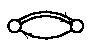
\includegraphics[width=0.26\textwidth]{figures/Fig_124_PDF227_Book215.pdf}
    \caption{练习 7.9(ii) 中的箭图（原书 p.215）}
    \label{fig:exercise-blowup-quiver}
  \end{figure}
  \item 证明相应的 $\widetilde{\mathbb A}^2$ 上的重言丛是一个倾斜丛。它的自同态环是什么？
\end{enumerate}
\end{exercise}

\begin{exercise}\label{exer:weighted-projective-line-stack}
考察带有群 $G=\{1,-1\}$ 作用的射影直线 $\mathbb P^1$，作用为
\[
  g\cdot(x:y)=(x:gy).
\]
加权射影直线 $\mathbb P^1_{2,2}$ 定义为商栈 $[\mathbb P^1/G]$。
\begin{enumerate}[label=(\roman*)]
  \item 定义 $\mathbb P^1_{2,2}$ 上 $G$-等变层的概念，并分类 $G$-等变线丛。令 $D\mathrm{Coh}^{\bullet}[\mathbb P^1/G]$ 表示 $G$-等变层的导出范畴。
  \item 将 $D\mathrm{Coh}^{\bullet}[\mathbb P^1/G]$ 解释为 $\mathbb P^1$ 上某个代数层的模所构成的导出范畴。
  \item 在 $D\mathrm{Coh}^{\bullet}[\mathbb P^1/G]$ 中寻找一个倾斜对象，并计算其自同态环。
\end{enumerate}
\end{exercise}

\chapterreview{%
\textbf{全章地位。}第 6 章用 Morse 理论造出 $A$ 侧的 $A_\infty$ 范畴，本章则用代数几何造出 $B$ 侧的相干层导出范畴与奇点范畴。作者避开消解与超上同调，改用仿射开集上的 Čech 复形直接给出 $A_\infty$ 增强，目的是让两侧范畴处在同一套语言里；第 8 至 10 章的镜像对应全部以 $D\mathrm{Coh}^{\bullet}X$ 为靶。

\textbf{知识脉络。}主线是“仿射环 $-$ 仿射簇反等价 $\to$ 模的层化 $\to$ 粘合成一般簇 $\to$ Čech 复形与层上同调 $\to$ 局部自由分解给出 $\mathrm{Perf}^{\bullet}X\subset D\mathrm{Coh}^{\bullet}X$”。§7.2 把机器推广到支撑层、概形、非交换簇、栈与 Landau--Ginzburg 模型；§7.3 反过来问导出范畴能记住多少几何：Fano 与反 Fano 簇可由 Serre 函子重构，一般簇之间的等价由 Fourier--Mukai 核给出，Orlov 定理说明这在光滑射影情形已完备；模空间与倾斜则把 $D\mathrm{Coh}^{\bullet}X$ 与箭图表示、$\mathrm{Perf}^{\bullet}A$ 联系起来。

\textbf{核心结论。}（1）仿射情形 $\mathrm{Perf}^{\bullet}X\cong_\infty D\mathrm{Proj}^{\bullet}R$，一般情形 $\mathrm{Perf}^{\bullet}X\subset D\mathrm{Coh}^{\bullet}X\subset D\mathrm{QCoh}^{\bullet}X$；$X$ 光滑当且仅当第一个包含是等价，也当且仅当 $D\mathrm{QCoh}^{\bullet}X$ 中 Hom 的次数有界。（2）矩阵分解由 $d_0d_1=d_1d_0=W$ 刻画：Knörrer 周期性给出 $\mathrm{MF}^{\pm}(R,W)\cong_\infty\mathrm{MF}^{\pm}(R[U,V],W+UV)$，孤立奇点情形由 Dyckerhoff 定理保证 $M_p$ 分裂生成，Buchweitz 定理把 $\mathrm{MF}^{0}(R,W)$ 等同于奇点范畴 $D^b\mathrm{Coh}X/\mathrm{Perf}X$。（3）仿射簇由 $\operatorname{End}(1_{D\mathrm{Coh}^{\bullet}X})\cong R$ 重构；Fano 或反 Fano 簇可由 Serre 函子 $-\otimes K[n]$ 重构。（4）核 $P\in D\mathrm{Coh}^{\bullet}(X\times Y)$ 给出 $\Phi_P=D\pi_{Y*}\circ(-\otimes P)\circ D\pi_X^*$，Orlov 定理断言光滑射影簇间的正合函子皆为此形；倾斜对象 $T$ 给出 $\mathcal C^{\bullet}\cong_\infty\mathrm{Perf}^{\bullet}A$，$A=\mathcal C^{\bullet}(T,T)$。

\textbf{辨析与提醒。}其一，$\bullet$ 记号不是装饰：$D\mathrm{Coh}^{\bullet}X$ 是 $A_\infty$ 增强，Hom 是复形而不仅是上同调群。其二，光滑性判据的方向要记清：光滑则每个相干层有有限局部自由分解，故 $\mathrm{Perf}=D\mathrm{Coh}$；有奇点时商 $D^b\mathrm{Coh}X/\mathrm{Perf}X$ 非零，它只探测奇点。其三，Serre 函子的自然同构方向极易写反，标准形式是 $\operatorname{Hom}(X,Y)\cong\operatorname{Hom}(Y,X\otimes K[n])^\vee$；Fourier--Mukai 的合成顺序同理，核在 $X\times Y$ 上决定函子 $X\to Y$，不能与转置核混为一谈。其四，$K^{-1}$ 丰富为 Fano、$K$ 丰富为反 Fano，方向只差一次对偶；“丰富”与“极丰富”也不同，后者要求 $L$ 本身给出射影嵌入。

\textbf{评注。}作者的取舍很明显：为与 $A$ 侧平行，他把层论压缩成“仿射覆盖 $+$ Čech 复形”，省略无界导出范畴的完备性、Brown 可表性与 Orlov 定理的证明；代价是补细节须另找文献，收益是 $B$ 侧范畴从第一页起就可计算。§7.2 把概形、栈与 LG 模型并置看似杂糅，实为第 8 章环簇与第 10 章镜像簇预置工具箱；矩阵分解若只当成 $\mathbb Z_2$ 玩具，就会错过它在分次理论中的核心地位。§7.3 揭示 $B$ 侧的刚性：Serre 函子把典范线丛变成范畴的内蕴对象，Fano 与反 Fano 因此可被范畴识别；到 Calabi--Yau 情形 $K$ 平凡，重构失效，镜像对应才真正开始。倾斜丛的存在性相当苛刻（例如所有射影 Calabi--Yau 簇都被排除），这也解释了作者为何把模空间与倾斜并置在末尾。阅读时宜与第 6 章对读：同一套 $A_\infty$ 语言，一侧由 Morse 轨迹给出，一侧由局部自由分解给出，这种对称是全书结构的主线。}
